%%% -*-LaTeX-*-
\chapter[Structural Inductive Biases for Observing Dialogue in \\
  Therapy]{Structural Inductive Biases for Observing Dialogue in
  Therapy}
\label{chap:snt}

Conversational agents have long been studied in the context of
psychotherapy, going back to chatbots such as
ELIZA~\citep{weizenbaum1966eliza} and
PARRY~\citep{colby1975artificial}. Research in modeling such dialogue
has largely sought to simulate a participant in the conversation.

In this chapter, we argue for modeling dialogue~\kw{observers} instead
of participants, and focus on psychotherapy\footnote{The main content
  of this chapter is published in~\citet{jie2019psycdialacl}}. An
observer could help an~\kw{ongoing} therapy session in several ways.
First, by monitoring fidelity to therapy standards, a helper could
guide both veteran and novice therapists towards better patient
outcomes. Second, rather than generating therapist utterances, it
could suggest the type of response that is appropriate. Third, it
could alert a therapist about potentially important cues from a
patient.
%
Such assistance would be especially helpful in the increasingly
prevalent online or text-based counseling services, e.g., Crisis Text
Line (\url{https://www.crisistextline.org}), 7 Cups
(\url{https://www.7cups.com}), etc.

We ground our study in a style of therapy called Motivational
Interviewing~\citep[MI,][]{miller2003motivational,miller2012motivational},
which is widely used for treating addiction-related problems.
%
To help train therapists, and also to monitor therapy quality,
utterances in sessions are annotated using a set of behavioral codes
called Motivational Interviewing Skill
Codes~\citep[MISC,][]{miller2003manual}. \autoref{tbl:bg:misc} shows
standard therapist and patient (\ie, client) codes with
examples. Recent NLP work~\cite[][{\em inter
  alia}]{tanana2016comparison, xiao2016behavioral,
  perez2017predicting, huang2018modeling} has studied the problem of
using MISC to assess~\emph{completed} sessions.  Despite its
usefulness, automated post hoc MISC labeling does not address the
desiderata for ongoing sessions identified above; such models use
information from utterances yet to be said. To provide real-time
feedback to therapists, we define two complementary dialogue
observers:
\begin{enumerate}[nosep]
\item \textbf{Categorization}: Monitoring an ongoing session by
  predicting MISC labels for therapist and client utterances as they
  are made.
\item \textbf{Forecasting}: Given a dialogue history, forecasting
  the MISC label for the next utterance, thereby both alerting or
  guiding therapists.
\end{enumerate}
Via these tasks, we envision a helper that offers assistance to a
therapist in the form of MISC labels.

We study modeling challenges associated with these tasks related to:
\begin{inparaenum}[(1)]
\item representing words and utterances in therapy dialogue,
\item ascertaining relevant aspects of utterances and the dialogue
  history, and
\item handling label imbalance (as evidenced in~\autoref{tbl:bg:misc}).
\end{inparaenum}
We develop neural models that address these challenges in this
domain.

Experiments show that our proposed models outperform baselines by a
large margin. For the categorization task, our models even outperform
previous session-informed approaches that use information from future
utterances. For the more difficult forecasting task, we show that even
without having access to an utterance, the dialogue history provides
information about its MISC label.  We also report the results of an
ablation study that shows the impact of the various design
choices.~\footnote{The code is available online at
  ~\url{https://github.com/utahnlp/therapist-observer}. The majority
  content of this chapter is published in our
  paper~\cite{jie2019psycdialacl}}.

In summary, in this chapter, we
\begin{inparaenum}[(1)]
\item factorize the dialog sequential structure via defining the tasks
  of categorizing and forecasting Motivational Interviewing Skill
  Codes to provide real-time assistance to therapists,
\item propose neural models for both tasks that outperform several
  baselines, and
\item show the impact of various modeling choices via extensive
  analysis.
\end{inparaenum}

\section{Background and Motivation}
\label{sec:snt:background}
Motivational Interviewing (MI) is a style of psychotherapy that
seeks to resolve a client's ambivalence towards their problems,
thereby motivating behavior change. Several meta-analyses and
empirical studies have shown the high efficacy and success of MI in
psychotherapy~\cite{burke2004emerging, martins2009review,
  lundahl2010meta}. However, MI skills take practice to master and
require ongoing coaching and feedback to
sustain~\cite{Schwalbe2014}.  Given the emphasis on using specific
types of linguistic behaviors in MI (\eg,
open questions and reflections), fine-grained behavioral coding
plays an important role in MI theory and training.

Motivational Interviewing Skill Codes (MISC, table~\ref{tbl:misc})
is a framework for coding MI sessions. It facilitates evaluating
therapy sessions via utterance-level labels that are akin to
dialogue acts~\cite{stolcke2000dialogue,jurafsky2018speech}, and are designed to examine therapist and client
behavior in a therapy session.\footnote{The original MISC description of
  \citet{miller2003manual} included 28 labels (9 client, 19
  therapist). Due to data scarcity and label confusion, various
  strategies are proposed to merge the labels into a coarser set.
  We adopt the grouping proposed by~\citet{xiao2016behavioral}; the
  appendix gives more details.}
% Like dialogue acts in general
% goal-oriented dialogue~\cite{jurafsky2018speech}, therapist codes
% characterize counselor and client behavior in a.
% Additionally, some therapist codes also mark the adherence to or
% against the spirit of MI. Client behavior
% codes are designed to characterize behavior change rather than the
% function of an utterance in the dialogue.

As Table~\ref{tbl:misc} shows,
client labels mark utterances as discussing changing or sustaining
problematic behavior (\CHANGE and \SUSTAIN, respectively) or being
neutral (\FN). Therapist utterances are grouped into eight labels,
some of which (\RES, \REC) correlate with improved outcomes, while
MI non-adherent (\MIN) utterances are to be avoided.  MISC labeling
was originally done by trained annotators performing multiple passes
over a session recording or a transcript.  Recent NLP work speeds up
this process by automatically annotating a completed MI
session~\cite[\eg,][]{tanana2016comparison, xiao2016behavioral,
  perez2017predicting}.

\emph{Instead of providing feedback to a therapist after the
  completion of a session, can a dialogue observer provide online
  feedback?} While past work has shown the helpfulness of post hoc
evaluations of a session, prompt feedback would be more helpful,
especially for MI non-adherent responses.  Such feedback opens up
the possibility of the dialogue observer influencing the therapy
session. It could serve as an assistant that offers suggestions to a
therapist (novice or veteran) about how to respond to a client
utterance. Moreover, it could help alert the therapist to
potentially important cues from the client (specifically, \CHANGE or
\SUSTAIN). % From a technical perspective, such real-time feedback
% poses similar challenges as the task of predicting dialogue intent
% in goal-oriented dialogue systems.



% In this paper, we are curious about whether NLP technologies can
%help in the above real-time setting. Although global ratings must be
%performed after an MI session finished, however, the utterance-level
%MISC code can be annotated in real-time as NLU component used to
%annotate dialogue intent in a goal-oriented dialogue system. Inspired
%but distinguished from current goal-oriented dialogue agent, we don't
%want to build a bot to substitute the therapist to chat with clients
%directly. Instead, we propose to build a novel third-party assistant
%agent, who not only can give rational judgement and alert to the
%therapist by monitoring what just happened in current dialogue, but
%also it can offer suggestion by forecasting the future
%conversation. According to the motivation above, we will first
%decompose and formulate the monitoring and forecasting ability into
%two seperate NLP tasks in \S\ref{sec:task}, then we describe our
%proposed models in \S\ref{sec:devices} and \S\ref{sec:models}.

%According to the manual of MISC~\cite{miller2003manual,
%houck2012motivational}, the original goal of MISC is to evaluate the
%quality of MI session, beyond the function of each utterance, the
%behavior codes also emphasize on 6 counselor rating dimensions:
%Acceptance, Empathy, Direction, Autonomy support, Collaboration, and
%Evocation, while the client MISC code are used to evaluate the target
%behavior change(TBC).\vs{The last sentence is too long. And it seems
%somewhat orthogonal}


%%% Local Variables:
%%% mode: latex
%%% TeX-master: "main"
%%% End:


\section[Independent Factorization for Motivational
Interviewing]{Independent Factorization for \\Motivational Interviewing}
\label{sec:snt:task}
In this section, we will formally define the two NLP tasks
corresponding to the vision in~\autoref{sec:snt:background} using the
conversation in~\autoref{tbl:snt:misc-example} as a running
example. Suppose we have an ongoing MI session with utterances
$u_1, u_2,\cdots, u_n$: together, the dialogue history $H_n$.  Each
utterance $u_i$ is associated with its speaker $s_i$, either C
(client) or T (therapist). We will define two classification tasks
over a fixed dialogue history with $n$ elements ---
\emph{categorization}~\autoref{ssec:snt:task-categorization} and
\emph{forecasting}~\autoref{ssec:snt:task-forecasting}.  Then we make a
comparative analysis on the independent factorization for the two
tasks~\autoref{ssec:snt:comparative-tasks}.

%We will refer to the last utterance $u_n$ as the \emph{anchor} for the
%corresponding subtasks.  As the conversation progresses, the history
%will be updated with a sliding window.  Since the therapist and client
%codes share no overlap, we will design separate models for the two
%speakers, giving us four settings in all.

\begin{table}[tbp]
  \caption{\label{tbl:snt:misc-example} An example of ongoing therapy session.}
  \begin{center}
    \setlength{\tabcolsep}{3pt}
    {
      \begin{tabular}{crll}
        \toprule
        \hline
        $i$        & $s_{i}$ & $u_{i}$                             & $l_{i}$  \\ \hline
        1        & T:      & Have you used drugs recently?       & \QUC     \\
        2        & C:      & I stopped for a year, but relapsed. & \FN      \\
        3        & T:      & You will suffer if you keep using. & \MIN     \\
        4        & C:      & Sorry, I just want to quit.         & \CHANGE  \\
        $\cdots$ &         & $\cdots$                            & $\cdots$ \\  \hline
        \bottomrule
      \end{tabular}
    }
  \end{center}
\end{table}

\subsection{Task 1: Categorization}
\label{ssec:snt:task-categorization}
The goal of this task is to provide real-time feedback to a
therapist during an ongoing MI session. In the running example, the
therapist's confrontational response in the third utterance is not
MI adherent (\MIN); an observer should flag it as such to bring the
therapist back on track. The client's response, however, shows an
inclination to change their behavior (\CHANGE). Alerting a therapist
(especially a novice) can help guide the conversation in a direction
that encourages it.

In previous posthoc dialogue analysis setting, we have the following
definition for the categorization task: \emph{Given the dialogue
  history $H_n=\{u_{1},u_{2}, ..., u_{n}\}$ which includes the speaker
  information, output a sequence of MISC label
  $L_n=\{l_{1}, l_{2}, ..., l_{n}\}$ for each utterance $u_i$.}

In essence, we have the following real-time classification task:
\emph{Given the dialogue history $H_n$ which includes the speaker
  information, predict the MISC label $l_n$ for the last utterance
  $u_n$.}

The key difference from previous work in predicting MISC labels is
that we are restricting the input to the real-time setting. As a
result, models can only use the dialogue history to predict the label,
and in particular, we can not use models such as a conditional random
field or a bidirectional LSTM that need both past and future inputs.

% \jc{I added this for comparing to
% previous dialogue act classification}
% \vs{I removed the content because it repeats information from
% section 3}

% For the client codes, it is similar to the sentiment analysis but it
% towards more on behavior changes, e.g., the client may feel happy
% and confident that smoking may help to relax, but this is \misc{NEG}
% in our cases. For therapist codes, this task can be considered as
% dialogue intent classification but emphasize professional counseling
% skills and spirits, such as empathy, support, and evocation.


\subsection{Task 2: Forecasting}
\label{ssec:snt:task-forecasting}
A real-time therapy observer may be thought of as an expert
therapist who guides a session with suggestions to the therapist.
For example, after a client discloses their recent drug use
relapse, a novice therapist may respond in a confrontational manner
(which is not recommended, and hence coded \MIN). On the other
hand, a seasoned therapist may respond with a complex reflection
(\REC) such as \dquoted{Sounds like you really wanted to give up and
  you're unhappy about the relapse.}
Such an expert may also anticipate important cues
from the client.% , expressing their intention to change or sustain
% their behavior
% .
The MISC forecasting task is a previously unstudied problem in the
posthoc dialogue analysis.

The forecasting task seeks to mimic the intent of such a seasoned
therapist: \emph{Given a dialogue history $H_n$ and the next speaker's
  identity $s_{n+1}$, predict the MISC code $l_{n+1}$ of the yet
  unknown next utterance $u_{n+1}$.}
% We
% argue that it is possible to learn to anticipate information about
% future utterances; this forms the basis of chatbot
% development.

We argue that forecasting the type of the next utterance, rather than
selecting or generating its text as has been the focus of several
recent lines of work~\citep[\eg,][]{schatzmann2005quantitative,lowe2015ubuntu,DSTC7},
allows the human in the loop~(the therapist) the freedom to
creatively participate in the conversation within the parameters
defined by the seasoned observer, and perhaps even rejecting
suggestions. Such an observer could be especially helpful for
training therapists~\citep{imel2017technology}.
%
The forecasting task is also related to recent work on detecting
antisocial comments in online
conversations~\citep{zhang2018conversations} whose goal is to
provide an early warning for such events.

\subsection[Independent Factorization for Categorization and
Forecasting Task]{Independent Factorization for Categorization \\and
  Forecasting Task}
\label{ssec:snt:comparative-tasks}

Take the dialogue segment in~\autoref{tbl:snt:misc-example} as a
running example, we compare the categorization and forecasting task
for each turn, with respect to the independent factorization for the
dialogue history and predicting target. Both categorization and
forecasting tasks are taking a sequence of dialogue utterances as
input, and then predict a sequence of MISC labels as output. They
share similar sequence labeling structures and seem to share the
same independent factorization. However, they have different
predicting goals when considering each dialogue turn. In the
following, we first introduce how we decompose the sequence of output
MISC labels according to the speaker, and then we present the
sliding window to decompose the input dialogue
history. \autoref{tbl:snt:task-comparasion} shows the clear
differences when we choose dialogue history window size as 3.

\subsubsection{Output Decomposition}
\label{sssec:snt:output-decomposition}
The outputs of both tasks are a sequence of MISC labels. Because each
MISC label is naturally associated with a corresponding utterance,
representing different functions as shown in
\autoref{tbl:bg:misc}. Hence for independent factorization, it is
natural to decompose the whole sequence prediction into a set of
continuous single MISC label prediction tasks as defined
previously. In such a way, each MISC prediction in the categorization
or forecasting task is independent of the MISC prediction in the
previous dialogue turn. However, they have different goals for each
dialogue turn. When the dialogue goes to turn 3, both the
categorization and forecasting task will observe the current dialogue
history window as input $X=H_{n}$. However, the key difference is as
follows: the categorization task is to predict the MISC code $l_{n}$
for the last seen utterance $u_{n}$, while the forecasting task is to
guess the future MISC code $l_{n+1}$ for the unseen utterance
$u_{n+1}$. To model this difference on output decomposition, we
introduce four components for dialogue and sentence representation
learning and search for the best model for each
task~\autoref{sec:snt:devices}. Furthermore, the MISC codes for the
clients and therapist represent different meanings and functions for
motivational skills. For example, the client MISC codes~( \SUSTAIN,
\CHANGE, and \FN) discuss the client's intention to change or sustain
problematic behavior or be neutral. While the therapist codes
represent the actions the therapist takes for a motivational
interview~(\eg, giving information~\GI, simple reflection~\RES). To
simplify the modeling, we also decompose the output according to the
speakers. For example, for the categorization task, we build two
models $C_{c}$ and $C_{t}$ for client and therapist codes
separately. Similar for the forecasting task, we study the $F_{c}$ and
$F_{t}$ for client and therapist. After such output decomposition,
every model only needs to classify on a unified set of MISC labels,
representing coherent goals for the clients or the therapist.

\subsubsection{Input Decomposition and Alignments Discovery}
\label{sssec:snt:input-decomposition}
For the input decomposition in previous lexical anchoring and phrasal
anchoring, the corresponding output label can be directly derived from
each input segment. For example, in lexical anchoring, each concept or
subgraph in an AMR graph is aligned to each token or special
entity. In phrasal anchoring, a nonterminal intent and slot label in
TOP is aligned to a phrase in the input sentence. In MISC code
prediction, the MISC code is assigned to a utterance. However, the
MISC code can not be derived by only a single token , phrase or the
aligned utterance. According to the MISC annotation guidedline, the
identification of relevant words or utterances may depend on the whole
dialogue history. For example, reflection related MISC~(\RES, \REC)
may need to discover which utterance in the dialogue history the
therapist are reflecting to. Hence, more than the previous
hard-aligned lexical-anchoring or phrasal-anchoring parsing, it
requires to discovering the relevant details in the meaning of the
sentence \textbf{within the context of dialogue history}. In
~\autoref{sec:snt:devices}, we proposed a hierarchical dialogue
encoder to model the nest structures of dialogue, and we also offered
word-level and utterance-level attention to help discover the relevant
parts in it.

Due to the realtime setting, the input dialogue is naturally
decomposed by time steps, and forms a sequence of incremental dialogue
history $\{u_1\}$, $\{u_1,u_2\}$, and $\{u_1,u_2,u_3\}$.  When the dialogue goes to the turn 4, the dialogue history will
slide to the next window of size 3, as $H_{n}=\{u_2,u_3,u_4\}$. The
$u_{1}$ will be truncated due the sliding window. We limit the
dialogue window because the whole therapy dialogue session may last
for 500 utterances, where current neural models such as RNN and
transformer can not handle the long context well.  In this dissertation
study~\autoref{ssec:snt:abl_context_attention}, we compare the window
size as 8 and 16 for our models. We leave the extremely long dialogue
context encoding as the future work.

\begin{table}[!tbp]
\caption{\label{tbl:snt:task-comparasion} The differences between the
  categorization task and the forecasting task, when choosing a window
  size as 3 to factorize the dialogue sequential flow.}
\begin{center}{
\setlength{\tabcolsep}{3pt}
\begin{tabular}{l|c|c|c}
\toprule
\hline
\multirow{2}{*}{Turn} & \multirow{2}{*}{$X=H_{n}$} & Categorization & Forecasting  \\
                      &                            & $Y=l_{n}$      & $Y=l_{n+1}$ \\ \hline
 1                    & $\{u_1\}$                  & {\QUC}         & {\FN}       \\
 2                    & $\{u_1,u_2\}$              & {\FN}          & {\MIN}      \\
 3                    & $\{u_1,u_2,u_3\}$          & {\MIN}         & {\CHANGE}   \\
 4                    & $\{u_2,u_3,u_4\}$          & {\CHANGE}      & {\RES}      \\ \hline
  \bottomrule
\end{tabular}}
\end{center}
\end{table}


%%% Local Variables:
%%% mode: latex
%%% TeX-master: "../../dissertation-main.ltx"
%%% End:


\section{Models for MISC Prediction}
\label{sec:snt:devices}

% \vs{General comment: For every section, add a label. I added one
%  above.}

% \vs{Rename the section title to be more descriptive: \eg, ``Modeling
% an Ongoing Dialogue'' or something else}

Modeling the two tasks defined in \S\ref{sec:task} requires
addressing four questions:
\begin{inparaenum}[(1)]
\item How do we encode a dialogue and its utterances?
\item Can we discover discriminative words in each utterance?
\item Can we discover which of the previous utterances are relevant?
\item How do we handle label imbalance in our data?
\end{inparaenum}
%
Many recent advances in % modeling dialogue with
neural networks can
be seen as plug-and-play components. To facilitate the comparative
study of models, we will describe components that address the
above questions.  % Then, we
% will compare the models and their various ablations as a combination
% of these modules in \S\ref{sec:experiments} and \ref{sec:analysis}
% respectively.
%
In the rest of the paper, we will use \textbf{boldfaced} terms to
denote vectors and matrices and \module{small caps} to denote
component names.



% In this section, for better comparative study on modeling
% psychotherapy dialogue our tasks, we first introduce thress
% plug-and-play components to study each of the following questions in
% our tasks. Then for each task, we will describe the best models and
% their ablations by representing it with a combinataion of these
% components in \S\ref{sec:models} and \ref{sec:analysis}.
%\vs{Don't use vague words like
%
%``some''. Be more concrete. Use a number. Here say ``four''. Also,
%  in other places in the paper.}  important
%\vs{\replaceWith{components to resolve each of the following
%    challenges}{design choices we need to address with respect to
%    modeling dialogue}}:
% \begin{enumerate}
% \item How to encode a dialogue and its utterances? (\S\ref{ssec:dialog_rep})
% \item How to capture important words for our tasks? (\S\ref{ssec:word_att})
% \item Can relevance between sentences help for our tasks? (\S\ref{ssec:sentence_att})
% \item How to handling label imbalance in our models ? (\S\ref{ssec:focal_loss})
% \end{enumerate}

% \vs{We spoke about the transfer learning point above.}
% \vs{Maybe these could be phrased as questions, and not in-para
% enum. That way, we could even add a reference to the subsection
% that discusses that question in parenthesis. The subsection titles
%  should use the words from the question. That way, it becomes easy
%  to read.}
%
%\begin{figure*}[t]
%\centering
%\includegraphics[width=0.3\textwidth]{hgru.png}\quad
%\includegraphics[width=0.3\textwidth]{gmlstm.png} \quad
%\includegraphics[width=0.3\textwidth]{multi-head.png} \quad
%\caption{\label{fig:models} (left) Hierarchical GRU, (middle) word-level Gated match-LSTM, (right) snt-level multi-head multi-hop self-attention. \vs{Do not use pngs if possible. Use pdf or eps}}
%\end{figure*}

\subsection{Encoding Dialogue}
\label{ssec:dialog_rep}

%\vs{See comment about subsection titles above}

%\vs{Start each subsection with a description of what the underlying problem is. Here, the problem is: To build any c%lassifier over a dialogue, we need to encode them into a vector form. Dialogues are sequences of utterences, which t% hemselves are sequences of tokens. This hierarchical structure has been widely studied in past work and the typical% approach is to use a hierarchical recurrent neural network [cite]...}

%Through extensive experiments in
%\S\ref{sec:experiments}, we find out the best combination of them for
%each task, and show what helps and what doesn't in each task with
%abalation studies in \S\ref{sec:analysis}.

Since both our tasks are classification tasks over a dialogue
history, our goal is to convert the sequence of utterences into a
single vector that serves as input to the final classifier.

We will use a hierarchical recurrent encoder~\cite[and
others]{li2015hierarchical,sordoni2015hierarchical,serban2016building}
to encode dialogues, specifically a hierarchical gated recurrent
unit (\HGRU) with an utterance and a dialogue encoder. We use a
bidirectional GRU over word embeddings to encode utterances. As is
standard, we represent an utterance $u_i$ by concatenating the final
forward and reverse hidden states. We will refer to this utterance
vector as $\bm{v}_i$. Also, we will use the hidden states of
each word as inputs to the attention components in
\S\ref{ssec:word_att}. We will refer to such contextual word
encoding of the $j^{th}$ word as $\bm{v}_{ij}$. The dialogue encoder
is a unidirectional GRU that operates on a concatenation of
utterance vectors $\bm{v}_i$ and a trainable vector representing the
speaker $s_i$.\footnote{For the dialogue encoder, we use a
  unidirectional GRU because the dialogue is incomplete. For words,
  since the utterances are completed, we can use a BiGRU.} The final
state of the GRU aggregates the entire dialogue history into a
vector $\bm{H}_n$.

% One way to encode a whole dialogue is concatenating all the dialogue
% utterances into a single long sentence and then encode it with a
% sequence encoder such as LSTM. However, it may lose important
% structure information of the dialogue after being flattened. Another
% widely used method is using hierarchical recurrent
% encoder~\cite{li2015hierarchical,
%   yang2016hierarchical,tang2015document, sordoni2015hierarchical,
%   serban2016building, tran2017hierarchical,
%   serban2017multiresolution}. In this paper, we adopt a hierarchical
%   GRU~(HGRU) as our model skeleton.

% An alternative to the \HGRU is to flatten the history into a
% sequence of utterences and use a single biGRU to encode this
% flattened history. We will refer to this strategy for encoding the
% dialogue history as \CON and denote the bidirectional encoding of
% the history as $\bm{C}$ and the hidden states of this BiGRU as
% $\bm{c}_1, \bm{c}_2, \cdots$.

The \HGRU skeleton can be optionally augmented with the
word and dialogue attention described next. All the models we will study are two-layer MLPs over the
vector $\bm{H}_n$ that use a ReLU hidden layer and a softmax layer
for the outputs.

%%% Local Variables:
%%% mode: latex
%%% TeX-master: "../../thesis-main.ltx"
%%% End:


\subsection{Word-level Attention}
\label{ssec:word_att}

Certain words in the utterance history are important to categorize or
forecast MISC labels. The identification of these words may depend on
the utterances in the dialogue. For example, to identify that an
utterance is a simple reflection (\RES) we may need to discover that
the therapist is mirroring a recent client utterance; the example
in table~\ref{tbl:misc} illustrates this. Word attention offers a
natural mechanism for discovering such patterns.

% Words are not equally important for our tasks. When classifying the
% current utterance $u_{n}$ in categorizing task, words in $u_{n}$ are
% usually more important than those in other utterances. For example,
% polarity and behavior related words ``quit'' in $u_{4}$ in Table
% ~\ref{tbl:example} are good indicators for \misc{NEG}, while most
% words in the dialogue history may be helpless. On the other side, only
% words in $u_{n}$ maybe not enough for identifying some codes. For
% example, only if words in $u_{n}$ are overlapping with previous
% utterances, then the label for $u_{n}$ is able about reflection~(e.g.,
% RES, REC, and REF). Hence, it is unclear whether word-attention can
% capture the above patterns.

We can unify a broad collection of attention mechanisms in NLP under
a single high level architecture~\cite{galassi2019attention}. We
seek to define attention over the word encodings $\bv_{ij}$ in the
history (called queries), guided by the word encodings in the anchor
$\bv_{nk}$ (called keys). The output is a sequence of
attention-weighted vectors, one for each word in the $i^{th}$
utterance.  The $j^{th}$ output vector $\ba_j$ is computed as a
weighted sum of the keys:
\begin{equation}
  \ba_{ij} = \sum_{k} \alpha^{k}_{j} \bv_{nk}
\label{eq:att_sum}
\end{equation}
The weighting factor $\alpha^k_j$ is the attention weight between
the $j^{th}$ query and the $k^{th}$ key, computed as
\begin{equation}
\label{eq:att_weight}
\alpha^{k}_{j} = \frac{\exp\left(f_{m}(\bv_{nk}, \bv_{ij})\right)}{\sum_{j^{\prime}} \exp\left(f_{m}(\bv_{nk}, \bv_{ij^\prime})\right)}
\end{equation}
Here, $f_m$ is a match scoring function between the corresponding
words, and different choices give us different attention mechanisms.

Finally, a combining function $f_{c}$ combines the original word
encoding $\bm{v}_{ij}$ and the above attention-weighted word vector
$\bm{a}_{ij}$ into a new vector representation $\bm{z}_{ij}$ as the final
representation of the query word encoding:
\begin{equation}
\bm{z}_{ij}= f_{c}(\bm{v}_{ij}, \bm{a}_{ij})
\end{equation}

The attention module, identified by the choice of the functions
$f_m$ and $f_c$, converts word encodings in each utterance
$\bv_{ij}$ into attended word encodings $\bm{z}_{ij}$. To use them
in the \HGRU skeleton, we will encode them a second time using a
BiGRU to produce attention-enhanced utterance vectors. For brevity,
we will refer to these vectors as $\bv_i$ for the utterance
$u_i$. If word attention is used, these attended vectors will be
treated as word encodings.


\begin{table}[t]
\begin{center}
  \setlength{\tabcolsep}{3pt}
  {\small
    \begin{tabular}{ll|l}
      \toprule
      Method                 & $f_{m} $                                    & $f_{c}$                                                             \\ \hline
      BiDAF                  & \multirow{2}{*}{$\bm{v}_{nk} {\bm{v}_{ij}^{T}}$}             & $[\bm{v}_{ij};~\bm{a}_{ij};  $                                      \\
                             &                                             & $~~\bm{v}_{ij} \odot \bm{a}_{ij};~\bm{v}_{ij}\odot \bm{a}^{\prime}]$ \\ \hline
      \multirow{2}{*}{GMGRU} & $\bm{w}^{e} \tanh(\bm{W}^{k}\bm{v}_{nk}$    & \multirow{2}{*}{$[\bm{v}_{ij};\bm{a}_{ij}]$}                        \\
                             & $~~+ \bm{W}^{q}[\bm{v}_{ij}; \bm{h}_{j-1}])$ &                                                                     \\ \hline
    \end{tabular}
  }
\end{center}
\caption{\label{tbl:word_att} Summary of word attention mechanisms.
  %
  We simplify BiDAF with multiplicative attention between  word
  pairs for $f_{m}$, while GMGRU uses additive attention
  influenced by the GRU hidden state.
  %
  The vector $\bm{w}_{e} \in\mathbb{R}^{d}$, and matrices
  $\bm{W}^{k}\in \mathbb{R}^{d \times d}$ and
  $\bm{W}^{q} \in\mathbb{R}^{2d \times 2d}$ are parameters of the BiGRU. The vector $\bm{h}_{j-1}$
  is the hidden state from the BiGRU in GMGRU at previous position
  $j-1$.  
  %
  For combination function, BiDAF concatenates bidirectional
  attention information from both the key-aware query vector
  $\ba_{ij}$ and a similarly defined query-aware key vector
  $\ba^{\prime}$. GMGRU uses simple concatenation for $f_c$.}
\end{table}

To complete this discussion, we need to instantiate the two
functions. We use two commonly used attention mechanisms:
BiDAF~\cite{bidaf} and gated matchLSTM~\cite{wang2017gated}. For
simplicity, we replace the sequence encoder in the latter with a
BiGRU and refer to it as GMGRU. Table~\ref{tbl:word_att} shows the
corresponding definitions of $f_{c}$ and $f_{m}$. We refer the
reader to the original papers for further details. In subsequent
sections, we will refer to the two attended versions of the \HGRU as
\BiDAFH and \GMGRUH.

% By specifying different sentence inputs as query and key, we summarize
% the inputs and outputs when using word-level attention over our
% skeleton CONCAT and HGRU dialogue encoding in Table
% \ref{tbl:word_att_q_key}. Worth to mention, we always involve the
% current utterance into dialogue history to weight with itself. Hence,
% it simultaneously captures the word interaction within the current
% utterance $n$ itself.

% \begin{table}[t]
% \begin{center}
% \setlength{\tabcolsep}{3pt}
% \begin{tabular}{lccc}
% \toprule
% Skeleton & Query   & Key  & Options\\ \hline 
% CON & $u_{n}$ & $C_{n}$ &  $\text{BiDAF}^{C}$,$\text{GMGRU}^{C}$ \\ 
% HGRU & $u_{i}$ & $u_{n}$ & $\text{BiDAF}^{H}$,$\text{GMGRU}^{H}
% $  \\ \bottomrule
% \end{tabular}
% \end{center}
% \caption{\label{tbl:word_att_q_key} For CON dialogue encoding, the
%   output of word attention is history-aware $u_{n}$ for
%   inference. While for HGRU, it output a query-aware history utterance
%   for each $u_{i}$. Then all the query-aware utterances will be
%   aggeragated by dialogue encoder to make a query-aware dialogue
%   representation $H_{n}$ for inference, }

% \end{table}

%In this paper, instead of inventing better attention mechanism for our tasks,
%we focused on to analysis how much word-level attention needed for our
%different task settings, and how it helps in our tasks. Hence, we
%choose to adopt a general gated extension from \cite{wang2017gated},
%where an extra gate was added to the input of the word attention
%aggregator to control how much attention in the vector $\bm{z}_{ij}$
%will be used when aggregating.
%
%\begin{equation}
%\bm{z}^{*}_{ij} = \text{sigmoid}(\bm{W}^{g}\bm{z}_{ij})\cdot\bm{z}_{ij}
%\end{equation}
%where $\bm{W}^{g} \in$

% % Match-LSTM is ported from textual % %entailment task to capture word-level
% attention between premise and %hypothesis.
% %In our model, we treat the response $r$
% as a premise and each %utterance in the
% dialogue history as a hypothesis. %


%\vs{I don't understand this paragraph at all. Please expand, with
%  equations if necessary. It should be accessible to those who
%  haven't read the match-LSTM paper.}

%\vs{Yes, equations will help. I don't understand what this is.}

%%% Local Variables:
%%% mode: latex
%%% TeX-master: "main"
%%% End:


\subsection{Utterance-Level Attention}
\label{ssec:sentence_att}
While we assume that the history of utterances is available for both
our tasks, not every utterance is relevant to decide a MISC label.
%
For categorization, the relevance of an utterance to the anchor may
be important. For example, a complex reflection (\REC) may depend on
the relationship of the current therapist utterance to one or more
of the previous client utterances. For forecasting, since we do not
have an utterance to label, several previous utterances may
be relevant. For example, in the conversation in
Table~\ref{tbl:snt:misc-example}, both $u_2$ and $u_4$ may be used to
forecast a complex reflection.

To model such utterance-level attention, we will employ the
multihead, multihop attention mechanism used in Transformer
networks~\citep{NIPS2017_7181}. As before, due to space constraints,
we refer the reader to the original work for details. We will use
the $(\bm{Q}, \bm{K}, \bm{V})$ notation from the original paper
here. These matrices represent a query, key and value,
respectively. The multihead attention is defined as:
%
\begin{equation}
\label{eq:multihead_attention}
{\small \text{Multihead}(\bm{Q},\bm{K},\bm{V}) = [\text{head}_{1};\cdots; \text{head}_{h}]\bm{W}^{O}}
\end{equation}
\begin{equation}
 \text{head}_{i} = \text{softmax}\left(\frac{\bm{Q}\bm{W}^{Q}_{i}\left(\bm{K}\bm{W}^{K}_{i}\right)^T}{\sqrt{d_{k}}}\right)\bm{V}\bm{W}^{V}_{i}
\end{equation}
The $\bm{W}_i$'s refer to projection matrices for the three inputs,
and the final $\bm{W}^o$ projects the concatenated heads into a
single vector.

The choices of the query, key and value defines the attention
mechanism. In our work, we compare two variants: {\em anchor-based
  attention}, and {\em self-attention}. The anchor-based attention
is defined by $Q = [\bm{v}_{n}]$ and
$K=V=[\bm{v}_{1} \cdots \bm{v}_{n}]$.  Self-attention is defined by
setting all three matrices to $[\bm{v}_{1} \cdots \bm{v}_{n}]$.
%
For both settings, we use four heads and stacking them for two hops,
and refer to them as $\self$ and $\anchor$.


%%% Local Variables:
%%% mode: latex
%%% TeX-master: "../../dissertation-main.ltx"
%%% End:



\subsection{Predicting and Training}
\label{ssec:inference_and_training}

From top to the bottom, every component will
produce some of useful representation for inferences in our tasks.
The dialogue encoding vector $\bm{H}_{n}$, as the final of the
unidirectional GRU, it is also the contextual utterance encoding
$\bm{h}_{u_{n}}$ of $u_{n}$. Hence $H_{n}$ can be directly used as a
representaion of $u_{n}$ for classification in annotating tasks, also
can be used as a represention of whole dialogue for forecasting
task. Hence in HGRU setting, we always use $\bm{H}_{n}$ as the base
option as input for inference.

However, for CON skeleton, the final state $C_{n}$ doest not exactly
represent the segement $u_{n}$ in the whole concatnated
dalogue. Hence, we concatenate the hidden state of the start
position~(0) and end position~(T) of $u_{n}$ into
$\bm{v}^{seg}_{n}=[h_{u^{0}_{n}};h_{u^{T}_{n}}]$, which is contextual
utterance encoding in CON mode.

Beside the above $\bm{H}_{n}$ and $\bm{C}_{n}$ contextual utterance
encoding in dialogue level, our components also produced the original
utterance encoding $\bm{v}_{n}$ from utterance encoder.  Whats'more,
in \textbf{CON} mode, we can use history-aware utterance encoding $\bm{v}^{wordatt}_{n}$
While in HGRU, it produced a self-attentive utterance encoding. We
denote it as $\bm{v}^{selfatt}_{n}$.

We summarize the option input encodings for inference
in~\autoref{tbl:inference_options}. There are two ways to scoring withthese
inputs, one is to score the concatenated those vectors together,
denoted as $\text{concat}(A, B)=\text{MLP}([A;B)$; The other one is
scoring each of them first and then add the scores up as the final
scores, such as $\text{add}(A,B)=\text{MLP}(A)+\text{MLP}(B)$.


\begin{table}[t]
\caption{\label{tbl:inference_options} Input options for annotating and forecasting tasks based on CON and HGRU skeletons.}
\begin{center}
\setlength{\tabcolsep}{3pt}
\begin{tabular}{lcc}
\toprule
Skeleton & Categorization & Forecasting  \\ \hline \hline
CON      & $\bm{v}^{seg}_{n}$,$\bm{v}^{{wordatt}_{n}}$, $\bm{v}_{n}$ & $\bm{C}_{n}$ \\ \hline
HGRU     & $\bm{H}_{n}$,$\bm{v}^{selfatt}_{n}$,$\bm{v}_{n}$          & $\bm{H}_{n}$ \\ \bottomrule
\end{tabular}
\end{center}
\end{table}


%%% Local Variables:
%%% mode: latex
%%% TeX-master: "../../dissertation-main.ltx"
%%% End:


\subsection{Addressing Label Imbalance}
\label{ssec:focal_loss}
From Table \ref{tbl:misc}, we see that both client and therapist
labels are imbalanced. Moreover, rarer labels are more important in
both tasks. For example, it is important to identify \CHANGE and
\SUSTAIN utterances. For therapists, it is crucial to flag MI
non-adherent (\MIN) utterances; seasoned therapists are trained to
avoid them because they correlate negatively with patient
improvements. If not explicitly addressed, the frequent but less
useful labels can dominate predictions.

% Previous
% work\cite{can2015dialog,tanana2016comparison, xiao2016behavioral}
% shows if not handing the label imbalance problem, results on client
% code may be dominated by most frequent label FN, and rarely predict POS
% and NEG; while for models on therapist codes, many of the rare labels,
% such as MIA, MIN will almost zero F1 score.
% One common solution for class imbalance is the $\alpha$-balanced
% cross entropy that weights different classes in standard cross
% entropy loss (CE) with $\alpha \in [0,1]$. Although easily
% classified labels may have small cross entropy value, the large
% number of them (for frequent labels) may still overwhelm the total
% cross entropy loss.

To address this, we extend the focal loss~\cite[FL][]{lin2017focal}
to the multiclass case. For a label $l$ with probability produced by
a model $p_t$, the loss is defined as 
\begin{equation}
 \label{eq:focal}
\text{FL}(p_{t}) = -\alpha_{t} {(1 -p_{t})}^{\gamma} \log(p_{t})
\end{equation}
In addition to using a label-specific balance weight $\alpha_t$, the
loss also includes a modulating factor ${(1-p_{t})}^{\gamma}$ to
dynamically downweight well-classified examples with
$p_{t}\gg0.5$. Here, the $\alpha_t$'s and the $\gamma$ are
hyperparameters. We use FL as the default loss function for all our
models.



%%% Local Variables:
%%% mode: latex
%%% TeX-master: "main"
%%% End:



%\subsection{Multiple Task Learning}
\label{ssec:mtl}

In this section, we studied whether the 4 settings in our tasks can benifit from each other.
To study the relation between annotating tasks ans forecasting task, we jointly learning the annotating tasks and forecasting task for the same speaker role as the C\_T and T\_JOINT.  To study, the relation between the client tasks and therapist task, we propose the alternative setting, our model alternative optimize for different tasks. Hence, we propose CT\_ANNO  and CT\_FORE for alternative learning for annotating tasks and forecasting task. Finally, we also proposed CT\_ALL for both alternative and jointly together, which learn our 4 settings all in one. We summerize our multple task learning settings in Table \ref{tbl:mtl}. Their experiment results are shown in Table \ref{tbl:mtl_result}

\begin{table}[tp]
\setlength{\tabcolsep}{3pt}
\begin{center}
\begin{tabular}{l|cc|cc}
\toprule
\hline
\multirow{2}{*}{ Method } & \multicolumn{2}{c|}{ Client } & \multicolumn{2}{c}{ Therapist } \\\cmidrule(lr){2-3}  \cmidrule(lr){4-5}
                          & Annotate                      & Forecast & Annotate & Forecast  \\ \midrule \midrule
C\_JOINT                  & Y                             & Y        &          &           \\
T\_JOINT                  &                               &          & Y        & Y         \\\midrule
CT\_ANNO                  & Y                             &          & Y        &           \\
CT\_FORE                  &                               & Y         &         & Y         \\ \midrule
CT\_ALL                   & Y                             & Y        & Y        & Y         \\ \hline
\bottomrule
\end{tabular}
\end{center}
\caption{\label{tbl:mtl} Summary of Multiple Task Learning on our paper}
\end{table}

%%% Local Variables:
%%% mode: latex
%%% TeX-master: "main"
%%% End:


%%% Local Variables:
%%% mode: latex
%%% TeX-master: "../../thesis-main.ltx"
%%% End:


\section{Experiments}
\label{sec:snt:experiments}

The original psychotherapy sessions were collected for both clinical
trials and Motivational Interviewing dissemination studies including
hospital settings~\citep{roy2014brief}, outpatient
clinics~\citep{baer2009agency}, college alcohol
interventions~\citep{tollison2008questions, neighbors2012randomized,
  lee2013indicated, lee2014randomized}.  All sessions were annotated
with the Motivational Interviewing Skills Codes (MISC)
\cite{atkins2014scaling}.  We use the train/test split of
\citet{can2015dialog, tanana2016comparison} to give 243 training MI
sessions and 110 testing sessions. We used 24 training sessions for
development.
% ~\footnote{\citet{can2015dialog, tanana2016comparison,
%     xiao2016behavioral} respectively use 111, 109, 101 sessions for
%   testing. After deduplication, we use 110 sessions, which are
%   almost the same with the first two papers.}
As mentioned in \S\ref{sec:snt:background}, all our experiments are
based on the MISC codes grouped by \citet{xiao2016behavioral}.


\subsection{Preprocessing and Model Setup}
\label{ssec:snt:exp_setup}
% The standard Motivational Interview Skill Codes (MISC)
% ~\cite{miller2003manual, houck2012motivational} contains 28 codes
% including 9 client codes and 19 therapist codes.  But some of them are
% too rare to build reasonable models. To address this issue, in
% previous works, several merging strategies have been proposed to group
% them into new categories \cite{can2015dialog, tanana2016comparison,
%   xiao2016behavioral}. In this paper, we follow the grouping strategy
% from \citet{xiao2016behavioral}. As shown in Table \ref{tbl:misc}, our
% dataset includes 3 client codes and 8 therapist codes.

%As shown in Table~\ref{tbl:misc}, for
%client codes, based on whether they are towards or away from to Target
%Behavior Change~(TBC), they are categorized into three codes: POS, NEG,
%and FN. Respectively, they represent the valence of changing,
%sustaining or following or neutral to the addictive behaviors
%~\cite{atkins2014scaling}. For therapist codes, we retain six original
%MISC code~(FA, GI, RES, REC, QUC, QUO). For other 13 rare codes,
%according to whether they represent MI adherent and MI non-adherent in
%the original MISC code annotation guideline, we cluster 8 of them into
%MIA and the other five into MIN. Table \ref{tbl:misc} shows the brief
%explanation and examples for final label set we used in our dataset
%and their distribution in our training corpus.
%% \vs{Too complicated para. Split somehow}

An MI session contains about 500 utterances on average. We use a
sliding window of size $N=8$ utterances with padding for the initial
ones. We assume that we always know the identity of the speaker for
all utterances. Based on this, we split the sliding windows into a
client and therapist windows to train separate models.
%
We tokenized and lower-cased utterances using
spaCy~\cite{spacy2}. To embed words, we concatenated 300-dimensional
Glove embeddings~\cite{pennington2014glove} with ELMo
vectors~\cite{Peters:2018}.

We use 300-dimensional Glove embeddings pre-trained on 840B tokens
from Common Crawl~\cite{pennington2014glove}. We do not update the
embedding during training. Tokens not covered by Glove are using a
randomly initialized UNK embedding. We also use character-level deep
contextualized embedding ELMo 5.5B model by concatenating the
corresponding ELMo word encoding after the word embedding vector. For
speaker information, we randomly initialize them with 8 dimensional
vectors and update them during training. We used a dropout rate of 0.3
for the embedding layers.

We trained all models using Adam~\cite{kingma2014adam} with learning
rate chosen by cross validation between $[1e^{-4}, 5*1e^{-4}]$,
gradient norms clipping from at $[1.0, 5.0]$, and minibatch sizes of
32 or 64. We use the same hidden size for both utterance encoder,
dialogue encoder and other attention memory hidden size; it has been
selected from $\{64, 128, 256, 512\}$. We set a smaller dropout 0.2
for the final two fully connected layers. All the models are trained
for 100 epochs with early-stoping based on macro $\text{F}_{1}$ over
development results.


% To
% simplify our model setting and simulate the realtime dialogue
% setting, for every dialogue utternace, imagining it as the most
% current utterance as dilogue goes on, then we only select its
% preceding $N$ utterances with their speaker and label information as
% our dialogue history(We use N= 8 for our main models, and use
% $N \leq 16$ for ablation study). We add padding empty utterances
% with special padding speaker and padding label ahead of the original
% context utterances when there is not enough preceding utterances.

% The speaker for every utterance is always given information, including
% the goal utterances, which are the last utterance to be categorized
% aid the future utterance to be forecasted\footnote{In real practise,
%   we don't know the future speaker, instead we forecast with models
%   for both client and therapist setting }. According to the speaker
% label of the goal utterances, we further split our dataset into client
% dataset and therapist dataset, and build seperate models for client
% and therapist on each of them respectively, which leads to reduced
% label confusion.

%%% Local Variables:
%%% mode: latex
%%% TeX-master: "../../dissertation-main.ltx"
%%% End:


\subsection{Results}
\label{ssec:snt:results}

Our goal is to discover the best client and therapist models for the
two tasks. We first summarize the best configuration and the
corresponding performance of our best models for both categorzing and
forecasting MISC codes in ~\autoref{tbl:main_rst} with precision,
recall and $F_{1}$ for each codes. Then, we also show the performance
of these models against various baselines.
\begin{table}[h]
\begin{center}
\setlength{\tabcolsep}{3pt}
\begin{tabular}{l|ccc|ccc}
\toprule
\hline
\multirow{2}{*}{{\bf Label}} & \multicolumn{3}{c}{{\bf Categorizing}} & \multicolumn{3}{c}{{\bf Forecasting}}  \\ \cline{2-4} \cline{5-7}
                             & P                                      & R    & $\text{F}_{1}$ & P    & R    & $\text{F}_{1}$ \\ \hline
\FN                          & 92.5                                   & 86.8 & 89.6    & 90.8 & 80.3 & 85.2    \\
\CHANGE                      & 34.8                                   & 44.7 & 39.1    & 18.9 & 28.6 & 22.7    \\
\SUSTAIN                     & 28.2                                   & 39.9 & 33.1    & 19.5 & 33.7 & 24.7    \\
\hline
\FA                          & 95.1                                   & 94.7 & 94.9    & 70.7 & 73.2 & 71.9    \\
\RES                         & 50.3                                   & 61.3 & 55.2    & 20.1 & 18.8 & 19.5    \\
\REC                         & 52.8                                   & 55.5 & 54.1    & 19.2 & 34.7 & 24.7    \\
\GI                          & 74.6                                   & 75.1 & 74.8    & 52.8 & 67.5 & 59.2    \\
\QUC                         & 80.6                                   & 70.4 & 75.1    & 36.2 & 24.3 & 29.1    \\
\QUO                         & 85.3                                   & 81.2 & 83.2    & 27.0 & 11.8 & 16.4    \\
\MIA                         & 61.8                                   & 52.4 & 56.7    & 27.0 & 10.6 & 15.2    \\
\MIN                         & 27.7                                   & 28.5 & 28.1    & 17.2 & 10.2 & 12.8    \\ \hline \bottomrule
\end{tabular}
\end{center}
\caption{Performance of our proposed
  models with respect to precision, recall and $\text{F}_{1}$ on categorizing and forecasting
  tasks for client and therapist codes}
\label{tbl:main_rst}
\end{table}

\Paragraph{Best Models} We identified the following best configurations using $\text{F}_{1}$
score on the development set:
\begin{enumerate}[nosep]
\item {\bf Categorization}: For client, the best model does not need any
  word or utterance attention. For the therapist, it uses \GMGRUH
  for word attention and \anchor for utterance attention. We refer
  to these models as $\mathcal{C}_C$ and $\mathcal{C}_T$ respectively
\item {\bf Forecasting}: For both client and  therapist, the best
  model uses no word attention, and uses \self utterance
  attention. We refer to these models as $\mathcal{F}_C$ and
  $\mathcal{F}_T$ respectively.
\end{enumerate}

\Paragraph{Results on Categorization}
Tables~\ref{tbl:main_rst_c_categorizing} and
\ref{tbl:main_rst_t_categorizing} show the performance of the
$\mathcal{C}_C$ and $\mathcal{C}_T$ models and the baselines.
%
For both therapist and client categorization, we compare the best
models against the same set of baselines. The majority baseline
illustrates the severity of the label imbalance
problem. \citet{xiao2016behavioral}, $\text{BiGRU}_{\text{generic}}$,
\citet{can2015dialog} and \citet{tanana2016comparison} are the
previous published baselines. The best results of previous published
baselines are underlined. The last row
$\Delta$ in each table lists the changes of our best model from
them. $\text{BiGRU}_{\text{ELMo}}$, $\text{CONCAT}^{C}$,
$\text{GMGRU}^{H}$ and $\text{BiDAF}^{H}$ are new baselines
we define below.

\begin{table}[!h]
\begin{center}{\small
\setlength{\tabcolsep}{3pt}
\begin{tabular}{lcccc}
\toprule
Method                                         & macro                & \FN                    & \CHANGE              & \SUSTAIN             \\ \midrule
% BiGRU(Xiao reported)                         & 48.5                 & 87.0                   & 30.0                 & 28.6                 \\
Majority                                       & 30.6                 & {\bf \underline{91.7}} & 0.0                  & 0.0                  \\
\citet{xiao2016behavioral}                     & 50.0                 & 87.9                   & 32.8                 & \underline{29.3}     \\
$\text{BiGRU}_{\text{generic}}$                & \underline{50.2}     & 87.0                   & \underline{35.2}     & 28.4                 \\
$\text{BiGRU}_{\text{ELMo}}$                   & 52.9                 & 87.6                   & {\bf 39.2}           & 32.0                 \\
\midrule
\citet{can2015dialog}                          & 44.0                 & 91.0                   & 20.0                 & 21.0                 \\
\citet{tanana2016comparison}                   & 48.3                 & 89.0                   & 29.0                 & 27.0                 \\
% CONCAT                                       & 49.9                 & 89.7                   & 32.1                 & 27.8                 \\
$\text{CONCAT}^{C}$                            & 51.8                 & 86.5                   & 38.8                 & 30.2                 \\
%$\text{GMGRU}^{C}$                            & 44.8                 & 24.4                   & 26.0                 & 83.9                 \\
%$\text{BiDAF}^{C}$                            & 44.8                 & 24.4                   & 26.0                 & 83.9                 \\
$\text{GMGRU}^{H}$                             & 52.6                 & 89.5                   & 37.1                 & 31.1                 \\
$\text{BiDAF}^{H}$                             & 50.4                 & 87.6                   & 36.5                 & 27.1                 \\ \midrule
%\citet{huang2018modeling}                     & -                    & -                      & -                    & -                    \\ \midrule
  $\mathcal{C}_{C}$                            & {\bf 53.9}           & 89.6                   & 39.1                 & {\bf 33.1}           \\
$\Delta=\mathcal{C}_{C} - \text{\underline{score}}$ & {\footnotesize +3.5} & {\footnotesize -2.1}   & {\footnotesize +3.9} & {\footnotesize +3.8} \\
  \bottomrule
\end{tabular}}
\end{center}
\caption{\label{tbl:main_rst_c_categorizing} Main results on categorizing
  client codes, in terms of macro $\text{F}_{1}$, and $\text{F}_{1}$ for
  each client code. Our model $\mathcal{C}_C$ uses final dialogue
  vector $H_{n}$ and current utterance vector $v_{n}$ as input of MLP
  for final prediction. We found that predicting using
  $\text{MLP}(H_{n})+\text{MLP}(v_{n})$ performs better than just
  $\text{MLP}({H_{n}})$.}
\end{table}

\begin{table}[!htp]
\begin{center}{\small
\begin{tabular}{lccccccccc}
\toprule
Method                                         & macro                & \FA                  & \RES                 & \REC             & \GI              & \QUC             & \QUO             & \MIA             & \MIN             \\ \midrule
Majority                                       & 5.87                 & 47.0                 & 0.0                  & 0.0              & 0.0              & 0.0              & 0.0              & 0.0              & 0.0              \\
\citet{xiao2016behavioral}                     & 59.3                 & \underline{94.7}     & 50.2                 & 48.3             & 71.9             & 68.7             & 80.1             & 54.0             & 6.5              \\
$\text{BiGRU}_{\text{generic}}$                & \underline{60.2}     & 94.5                 & \underline{50.5}     & \underline{49.3} & 72.0             & 70.7             & 80.1             & \underline{54.0} & \underline{10.8} \\
$\text{BiGRU}_{\text{ELMo}}$                   & 62.6                 & 94.5                 & 51.6                 & 49.4             & 70.7             & 72.1             & 80.8             & 57.2             & 24.2             \\ \midrule
\citet{can2015dialog}                          & -                    & 94.0                 & 49.0                 & 45.0             & \underline{74.0} & \underline{72.0} & \underline{81.0} & -                & -                \\
\citet{tanana2016comparison}                   & -                    & 94.0                 & 48.0                 & 39.0             & 69.0             & 68.0             & 77.0             & -                & -                \\
$\text{CONCAT}^{C}$                            & 61.0                 & 94.5                 & 54.6                 & 34.3             & 73.3             & 73.6             & 81.4             & 54.6             & 22.0             \\
%$\text{GMGRU}^{C}$                            & 41.0                 & 92.4                 & 19.7                 & 39.1             & 65.1             & 39.4             & 65.0             & 7.4              & 0.0              \\
%$\text{BiDAF}^{C}$                            & 38.0                 & 90.7                 & 22.0                 & 19.4             & 62.5             & 41.9             & 61.2             & 6.5              & 0.0              \\
$\text{GMGRU}^{H}$                             & 64.9                 & 94.9                 & {\bf 56.0}           & 54.4             & {\bf 75.5}       & {\bf 75.7}       & {\bf 83.0}       & {\bf 58.2}       & 21.8             \\
$\text{BiDAF}^{H}$                             & 63.8                 & 94.7                 & 55.9                 & 49.7             & 75.4             & 73.8             & 80.7             & 56.2             & 24.0             \\ \midrule
%\citet{huang2018modeling}                     & -                    & -                    & -                    & -                & -                & -                & -                & -                &                  \\ \midrule
$\mathcal{C}_{T}$                              & {\bf 65.4}           & {\bf 95.0}           & 55.7                 & {\bf 54.9}       & 74.2             & 74.8             & 82.6             & 56.6             & {\bf 29.7}       \\
$\Delta=\mathcal{C}_{T} - \text{\underline{score}}$ & {\footnotesize +5.2} & {\footnotesize +0.3} & {\footnotesize +3.9} & {\footnotesize +3.8} & {\footnotesize +0.2} & {\footnotesize +2.8} & {\footnotesize +1.6} & {\footnotesize +2.6} & {\footnotesize +18.9}                                                                                                \\ \bottomrule
\end{tabular}}
\end{center}
\caption{\label{tbl:main_rst_t_categorizing} Main results on
  categorizing therapist codes, in terms of macro $\text{F}_{1}$, and
  $\text{F}_{1}$ for each therapist code. Models are the same as Table
  ~\ref{tbl:main_rst_c_categorizing}, but tuned for therapist
  codes. For the two grouped MISC set \MIA and \MIN, their results are
  not reported in the original work due to different setting.}
\end{table}



The first set of baselines (above the line) do not encode dialogue
history and use only the current utterance encoded with a BiGRU. The
work of \citet{xiao2016behavioral} falls in this category, and uses a
100-dimensional domain-specific embedding with weighted cross-entropy
loss. Previously, it was the best model in this class. We also
re-implemented this model to use either ELMo or Glove vectors with
focal loss.\footnote{Other related work in no context
  exists~\cite[e.g.,][]{perez2017predicting, gibson2017attention}, but
  they either do not outperform \cite{xiao2016behavioral} or use
  different data.}

The second set of baselines (below the line) are models that use
dialogue context.  Both \citet{can2015dialog} and
\citet{tanana2016comparison} use well-studied linguistic features and
then tagging the current utterance with both past and future utterance
with CRF and MEMM, respectively. To study the usefulness of the
hierarchical encoder, we implemented a model that uses a bidirectional
GRU over a long sequence of flattened utterance. We refer to this as
$\text{CONCAT}^{C}$. This model is representative of the work
of~\citet{huang2018modeling}, but was reimplemented to take advantage
of ELMo.



% (superscript
% $C$ means categorizing, for distinguishing models for forecasting
% task) is based on the CON skeleton, which use BIGRU to encode a
% concatenated dialogue history and use the output history encoding as
% extra features for classification. It contributes the main improvement
% in~\citet{huang2018modeling}~\footnote{ \citet{huang2018modeling}
%   studied categorizing only client codes on a different dataset. For
%   comparison, we reimplement the $\text{CONCAT}^{C}$ method with ELMo
%   in our paper, and also studied their proposed input add-ons
%   separately in \S\ref{ssec:abl_context_attention}, and we leave topic
%   model embedding as our future work.  }

For categorizing client codes, $\text{BiGRU}_{\text{ELMo}}$ is a
simple but robust baseline model. It outperforms the previous
best no-context model by more than 2 points on macro $\text{F}_{1}$. Using the
dialogue history, the more sophisticated model $\mathcal{C}_{C}$
further gets 1 point improvement. Especially important is its
improvement on the infrequent, yet crucial labels \CHANGE and
\SUSTAIN. It shows a drop in the $\text{F}_{1}$ on the \FN label, which is
essentially considered to be an unimportant, background class from
the point of view of assessing patient progress.
%
For therapist codes, as the highlighted numbers in Table
\ref{tbl:main_rst_t_categorizing} show, only incorporating GMGRU-based
word-level attention, $\text{GMGRU}^{H}$ has already outperformed many
baselines, our proposed model $\mathcal{F}_{T}$ which uses both
GMGRU-based word-level attention and anchor-based multi-head multihop
sentence-level attention can further achieve the best overall
performance. Also, note that our models outperform approaches
that take advantage of future utterances.

For both client and therapist codes, concatenating dialogue history
with $\text{CONCAT}^{C}$ always performs worse than the hierarchical
method and even the simpler $\text{BiGRU}_{\text{ELMo}}$.

\begin{table}[!h]
\centering
\begin{tabular}{lcccccc}
  \toprule
  \multirow{2}{*}{Method} & \multicolumn{2}{c}{Dev} & \multicolumn{4}{c}{Test}                                       \\ \cmidrule(lr){2-3} \cmidrule(lr){4-7}
                          & \CHANGE                 & \SUSTAIN   & macro      & \FN        & \CHANGE    & \SUSTAIN   \\ \midrule \midrule
%  BiGRU                  &                         &            &            &            &            &            \\
$\text{CONCAT}^{F}$       & 20.4                    & 30.2       & 43.6       & 84.4       & 23.0       & {\bf 23.5} \\
% CONCAT(no ELMo)         & 27.4                    & 18.0       & 36.6       & {\bf 87.7} & 18.5       & 18.2       \\
  HGRU                    & 19.9                    & 31.2       & {\bf 44.4} & 85.7       & {\bf 24.9} & 22.5       \\
  $\text{GMGRU}^{H}$      & 19.4                    & 30.5       & 44.3       & 87.1       & 23.3       & 22.4       \\ \midrule
%  $\text{GMGRU}^{C}$     & 8.7                     & 28.5       & 40.4       & 87.0       & 11.7       & 22.6       \\
  $\mathcal{F}_{C}$       & {\bf 21.1}              & {\bf 31.3} & 44.3       & 85.2       & 24.7       & 22.7       \\
\bottomrule
\end{tabular}
\caption{\label{tbl:main_rst_forecast:client} Main results on forecasting client codes, in terms of $\text{F}_{1}$ for \SUSTAIN, \CHANGE on dev set, and macro $\text{F}_{1}$, and $\text{F}_{1}$ for each client code on the test set.}
\end{table}

\begin{table}[!h]
\centering
\begin{tabular}{ccccccccccc}
\toprule
\multirow{2}{*}{Method} & \multicolumn{1}{c}{Recall} & \multicolumn{9}{c}{$\text{F}_{1}$}                                                                                             \\ \cmidrule(lr){2-2} \cmidrule(lr){3-11}
                        & R@3                        & macro      & \FA        & \RES       & \REC       & \GI        & \QUC       & \QUO       & \MIA       & \MIN       \\ \midrule \midrule
% BiGRU                 &                            &            &            &            &            &            &            &            &            &            \\
% CONCAT                & 72.0                       & 22.0       & 63.2       & 2.6        & 14.5       & 52.8       & 24.9       & 5.5        & 12.0       & 0.0        \\
$\text{CONCAT}^{F}$     & 72.5                       & 23.5       & 63.5       & 0.6        & 0.0        & 53.7       & 27.0       & 15.0       & 18.2       & 9.0        \\
% HGRU_generic          & 76.8                       & 24.0       & 71.0       & 2.7        & 20.5       & 58.8       & 27.5       & 12.9       & {\bf 15.2} & 1.6        \\
HGRU                    & 76.0                       & 28.6       & 71.4       & 12.7       & {\bf 24.9} & 58.3       & 28.8       & 5.9        & {\bf 17.4} & 9.7        \\
$\text{GMGRU}^{H}$      & 76.6                       & 26.6       & {\bf 72.6} & 10.2       & 20.6       & 58.8       & 27.4       & 6.0        & 8.9        & 7.9        \\ \midrule
%$\text{GMGRU}^{C}$     & 67.6                       & 19.6       & 62.0       & 11.8       & 19.7       & 51.6       & 10.0       & 1.9        & 0.1        & 0.0        \\ \midrule
$\mathcal{F}_{T}$       & {\bf 77.0}                 & {\bf 31.1} & 71.9       & {\bf 19.5} & 24.7       & {\bf 59.2} & {\bf 29.1} & {\bf 16.4} & 15.2       & {\bf 12.8} \\
\bottomrule
\end{tabular}
\caption{\label{tbl:main_rst_forecast:therapist} Main results on forecasting therapist codes, in terms of Recall@3, macro $\text{F}_{1}$, and $\text{F}_{1}$ for each label on test set}
\end{table}

\Paragraph{Results on Forecasting} Since the forecasting task is
new, there are no published baselines to compare against. Our
baseline systems essentially differ in their representation of
dialogue history. The model $\text{CONCAT}^{F}$ uses the same
architecture as the model $\text{CONCAT}^{C}$ from the categorizing
task. We also show comparisons to the simple \HGRU model and the
\GMGRUH model that uses a gated matchGRU for word
attention.\footnote{The forecasting task bears similarity to the
  next utterance selection task in dialogue state tracking
  work~\cite{DSTC7}. In preliminary experiments, we found that the
  Dual-Encoder approach used for that task consistently
  underperformed the other baselines described here.}

\autoref{tbl:main_rst_forecast:client} and
\autoref{tbl:main_rst_forecast:therapist} show our forecasting results
for client and therapist respectively. For client codes, we also
report the \CHANGE and \SUSTAIN performance on the development set
because of their importance.  For the therapist codes, we also report
the recall@3 to show the performance of a suggestion system that
displayed three labels instead of one.
%
The results show that even without an utterance, the dialogue history
conveys signal about the next MISC label. Indeed, the performance for
some labels is even better than some categorization baseline
systems. Surprisingly, word attention ($\text{GMGRU}^{H}$) in both
the~\autoref{tbl:main_rst_forecast:client} and
\autoref{tbl:main_rst_forecast:therapist} did not help in forecasting
setting, and a model with the \self utterance attention is
sufficient. For the therapist labels, if we always predicted the three
most frequent labels (\FA, \GI, and \RES), the recall@3 is only 67.7,
suggesting that our models are informative if used in this
suggestion-mode.

%%% Local Variables:
%%% mode: latex
%%% TeX-master: "../../thesis-main.ltx"
%%% End:


%%% Local Variables:
%%% mode: latex
%%% TeX-master: "../../thesis-main.ltx"
%%% End:


\section{Analysis and Ablations}
\label{sec:snt:analysis}
This section reports error analysis and an ablation study of our
models on the development set. The appendix shows a comparison of
pretrained domain-specific ELMo/glove with generic ones and the
impact of the focal loss compared to simple or weighted
cross-entropy.

\subsection{Label Confusion and Error Breakdown}
\label{ssec:label_confusion}
% The MISC annotation guidelines~\cite{miller2003manual,
%   houck2012motivational} lists labels that are known to be easily confused.

%   with each other except between \GI, \QUO, \QUC.

Figure \ref{fig:categorizing_confusion_client} shows the confusion
matrix for the client categorization task. The confusion between \FN
and \CHANGE/\SUSTAIN is largely caused by label imbalance. There are 414 \CHANGE examples that are predicted as \SUSTAIN
and 391 examples vice versa. To further understand their confusion, we
selected 100 of each for manual analysis. We found four broad
categories of confusion, shown in Table
\ref{tbl:c_client_errors}.

\begin{figure}[!tbp]
\begin{center}
  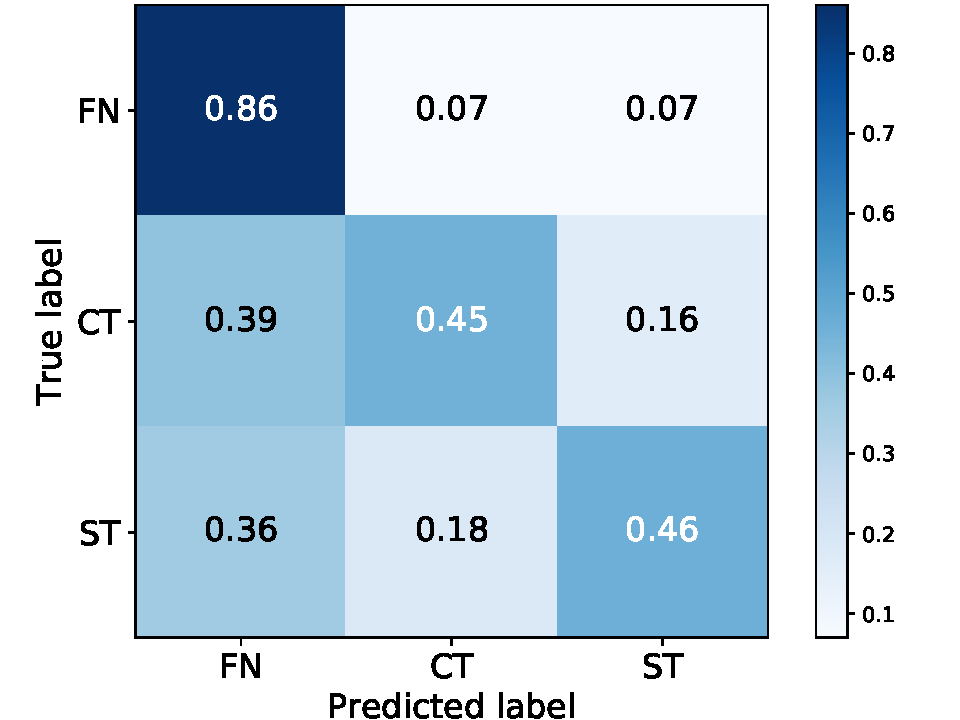
\includegraphics[width=0.50\textwidth]{large_font_categorizing_plabel_confusion_matrix_dev.pdf}
\end{center}
  \caption{\label{fig:categorizing_confusion_client} Confusion matrix for categorizing client codes, normalized by row.}
\end{figure}

\begin{table}[!h]
\caption{Categorization of \CHANGE/\SUSTAIN confusions.The two numbers in the brackets are the count of errors for predicting \CHANGE as \SUSTAIN and vice versa. We exampled 100 examples for each case.}
  \small
  \begin{center}
\begin{tabular}{ll}
  \toprule
  \hline
  {\bf Category and Explaination}                                                                                                                                                                                                                            & {\bf Client Examples (Gold MISC)}                                                                                                                                         \\\midrule
  \multirow{4}{*}{\parbox{7cm}{Reasoning is required to understand
  whether a client wants to change behavior, even with full context~(50,42) }}                               & \multirow{4}{*}{\parbox{7cm}{T: On a scale of zero to ten how confident are you that you can implement this change? \\C: I don't know, seven maybe (\CHANGE);\\ I have to wind down after work (\SUSTAIN) }} \\
                                                                                                                                                                                                                                                             &                                                                                                                                                                     \\
                                                                                                                                                                                                                                                             &                                                                                                                                                                     \\
                                                                                                                                                                                                                                                             &                                                                                                                                                                     \\\midrule
  \multirow{4}{*}{\parbox{7cm}{Concise utterances which are easy for humans to understand, but missing information such as coreference, zero pronouns~(22,31)}}                                                                                        & \multirow{4}{*}{\parbox{7cm}{I mean I could try it (\CHANGE)\\Not a negative consequence for me (\SUSTAIN) \\I want to get every single second and minute out of it(\CHANGE)}}                                                                                                                                     \\
                                                                                                                                                                                                                                                             & \\
                                                                                                                                                                                                                                                             & \\
                                                                                                                                      & \\\midrule
  \multirow{3}{*}{\parbox{7cm}{Extremely short ($ \leq5 $) or long sentence ($\ge40 $), caused by incorrect turn segementation. ~(21,23)}} & It is a good thing (\SUSTAIN)                                   \\
                                                                                                                                      & Frankly, I hate it (\CHANGE)                                                               \\ & Painful (\CHANGE)                                                                                                                                                    \\ \midrule
  \multirow{2}{*}{\parbox{7cm}{Ambivalent speech, very hard to understand even for human.~(7,4)}}                                     & \multirow{3}{*}{\parbox{7cm}{What if it does n't work I mean what if I can't do it (\SUSTAIN)\\But I can stop whenever I want(\SUSTAIN)}}                                                                                                                            \\
& \\                                                                                                                                                                                                                                                             &                                                                                                                             \\ \hline
\bottomrule
\end{tabular}
\end{center}
\label{tbl:c_client_errors}
\end{table}

The first category requires more complex reasoning than just surface
form matching. For example, the phrase \example{seven out of ten}
indicates that the client is very confident about changing behavior;
the phrase \example{wind down after work} indicates, in this context,
that the client drinks or smokes after work. We also found that the
another frequent source of error is incomplete information. In a
face-to-face therapy session, people may use concise and effient
verbal communication, with guestures and other body language conveying
information without explaining details about, for example,
coreference.  With only textual context, it is difficult to infer the
missing information. The third category of errors is introduced when
speech is transcribed into text. The last category is about ambivalent
speech. Discovering the real attitude towards behavior change behind
such utterances could be difficult, even for an expert therapist.
% \todo{@Vivek, I found this is interesting but
%   not easy to write in professoinal linguistic term, please help to revise}
%\begin{table}[!htbp]
%\begin{center}
%\setlength{\tabcolsep}{5pt}
%\begin{tabular}{c|c|c}
%\toprule
%Label & Confusion Label Set          & Model2T & Kappa\\
%\midrule
%FA    & \RES, \REC, GI, QUC, QUO, MIA(Structure), MIN(Confront)                \\
%\RES   & FA, \REC, GI, QUC,QUO, MIA(Affirm, Emphasize Control), MIN(Confront)     \\
%\REC   & FA, \RES, GI, QUC,QUO, MIA(Affirm, Emphasize Control), MIN(Confront)   \\
%GI    & FA, \RES, \REC, MIA(ADP), MIN(Confront, Warn, Direct)                \\
%QUC   & FA,\RES, \REC,QUO,MIA(ADW), MIN          \\
%QUO   & FA,\RES, \REC,QUC,MIA(ADW), MIN         \\
%MIA   & FA, \RES, \REC, GI,QUO,QUC, MIN(ADW)                 \\
%MIN   & FA, \RES. \REC,GI,QUC,QUO,MIA(ADP) \\
%\bottomrule
%\end{tabular}
%\end{center}
%\caption{\label{tbl:confusion_guide} Confusing label set for each label from the MISC Annotation guidelines}
%\end{table}
\begin{figure}[!tbp]
\begin{center}
  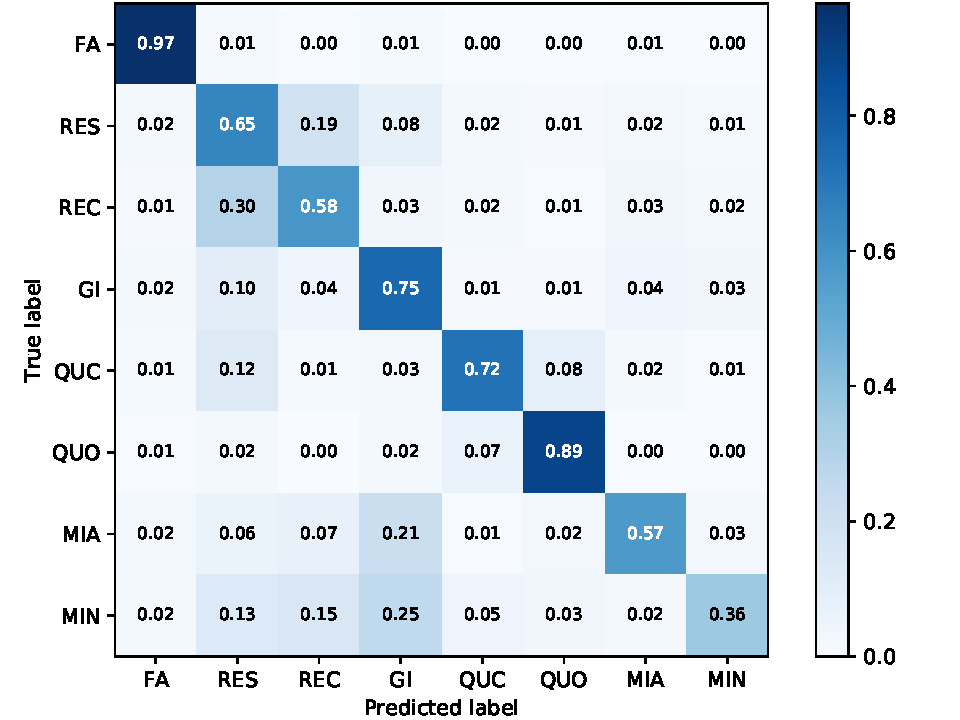
\includegraphics[width=0.90\textwidth]{pred_tlabel_model2_confusion_dev.pdf}
\end{center}
  \caption{\label{fig:categorizing_confusion_therapist} Confusion matrix for categorizing therapist codes, normalized by row.}
\end{figure}

Figures~\ref{fig:categorizing_confusion_client} and~\ref{fig:categorizing_confusion_therapist} show the
label confusion matrices for the best categorization models. We will
examine confusions that are not caused purely by a label being
frequent. We observe a common confusion between
the two reflection labels, \REC and \RES. Compared to the
confusion matrix from \citet{xiao2016behavioral}, we see that our
models show much-decreased confusion here. There are two reason for
this confusion persisting. First, the reflections may require a much
longer information horizon. We found that by increasing the window
size to 16, the overall reflection results improved. Second, we need
to capture richer meaning beyond surface word overlap for
\RES. We found that
complex reflections usually add meaning or emphasis  to
previous client statements using devices such as analogies,
metaphors, or similes rather than simply restating them. % Hence, it requires much other analysis
% more than attention-based word-overlapping.

%
Closed questions (\QUC) and simple reflections (\RES) are known to
be a confusing set of labels. For example, an utterance like
\tquoted{Sounds like you're suffering?} may be both.
%
Giving information (\GI)
is easily confused with many labels because they relate to providing
information to clients, but with different attitudes. The MI adherent
(\MIA) and nonadherent (\MIN) labels may also provide information,
but with supportive or critical attitude that may be difficult to
disentangle, given the limited number of examples.


%\begin{figure}[!htbp]
%\centering
%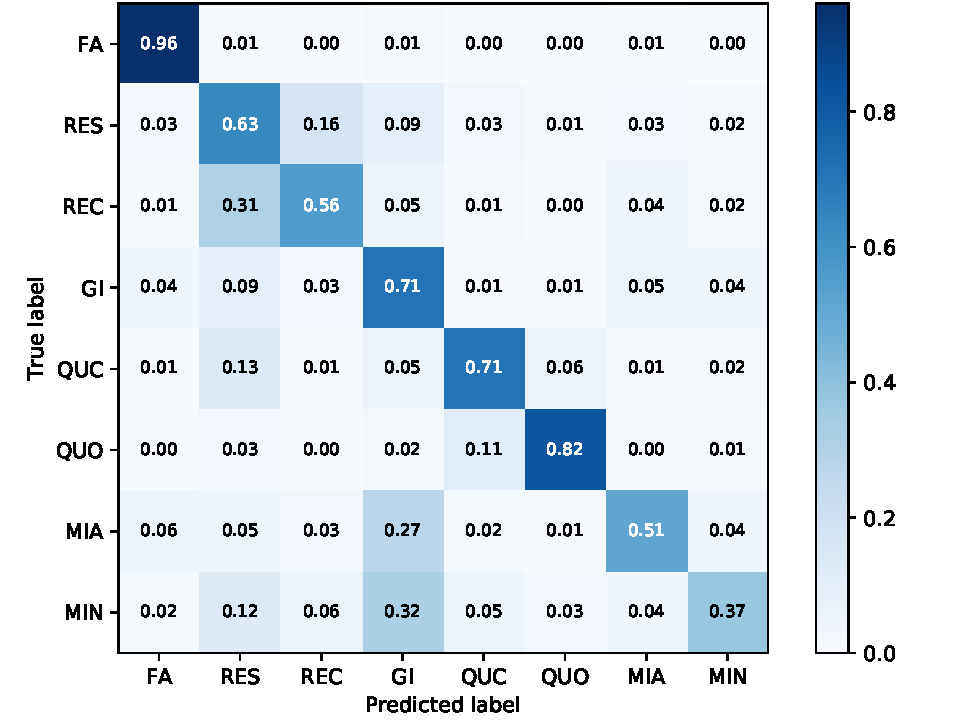
\includegraphics[width=0.5\textwidth]{pred_tlabel_model2_confusion.png}
%\caption{\label{fig:categorizing_t_confusion} Normalized label confusion matrix for categorizing therapist code.}
%\end{figure}

%%% Local Variables:
%%% mode: latex
%%% TeX-master: "../../dissertation-main.ltx"
%%% End:


\subsection{How Context and Attention Help?}
\label{ssec:snt:abl_context_attention}

We evaluated various ablations of our best models to see how
changing various design choices changes performance. We focused on
the context window size and impact of different word level and
sentence level attention mechanisms. Tables \ref{tbl:rst_cxt_client}
and \ref{tbl:rst_cxt_therapist} summarize our results.

\subsubsection{History Size}
\label{sssec:snt:history-size}
Increasing the history window size generally helps. The biggest
improvements are for categorizing therapist codes
(Table~\ref{tbl:rst_cxt_therapist}), especially for the \RES and
\REC. However, increasing the window size beyond 8 does not help
to categorize client codes~(\autoref{tbl:rst_cxt_client}) or
forecasting~(\autoref{tbl:rst_cxt_forcasting}).

\begin{table}[t]
  \caption{\label{tbl:rst_cxt_forcasting} Ablation study on
    forecasting task on both client and therapist code. $*$ row are
    results of our best forecasting model $\mathcal{F}_{C}$, and
    $\mathcal{F}_{T}$.  $\setminus$ means substitute anchor attention with
    self attention. $+\text{GMGRU}$ \anchor means using word-level
    attention and achor-based sentence-level attention
    together. Word-level attention shows no help for both client and
    therapist codes. While sentence-level attention helps more on
    therapist codes than on client codes. Multi-head self attention
    also achieves better performance than anchor-based attention in
    forecasting tasks. }
\begin{center}
\setlength{\tabcolsep}{2.5pt}
{\small
\begin{tabular}{ccccccccccccc}
\toprule
Ablation                                                               & Options               & \CHANGE    & \SUSTAIN   & R@3        & \FA        & \RES       & \REC       & \GI        & \QUC       & \QUO       & \MIA       & \MIN       \\ \midrule \midrule
\multirow{4}{*}{\parbox{1.5cm}{history size}}                          & 1                     & 17.2       & 15.1       & 66.4       & 59.4       & 12.6       & 9.0        & 44.6       & 16.3       & 14.8       & 11.9       & 4.1        \\
                                                                       & 4                     & 16.8       & 22.6       & 75.3       & 71.4       & 15.6       & 21.1       & 57.1       & {\bf 29.3} & 11.0       & 11.2       & 14.4       \\
                                                                       & $8^{*}$               & 24.7       & 22.7       & {\bf 77.0} & {\bf 72.8} & {\bf 20.8} & 23.1       & 58.1       & 28.3       & {\bf 17.7} & 15.9       & 9.0        \\
                                                                       & 16                    & 23.9       & 20.7       & 76.5       & 71.2       & 13.7       & 24.1       & {\bf 58.5} & 25.9       & 9.7        & 16.2       & 12.7       \\ \midrule
\multirow{2}{*}{\parbox{1.5cm}{\parbox{1.5cm}{word \quad\quad attention}}}     & GMGRU                 & 14.0       & {\bf 23.2} & 75.7       & 71.7       & 14.2       & 23.0       & 57.5       & 26.5       & 8.0        & 15.4       & 11.6       \\
                                                                       & $\text{GMGRU}_{4h}$   & 19.1       & 22.9       & 76.3       & 71.3       & 12.1       & 23.3       & 58.1       & 24.5       & 12.6       & 11.7       & 14.0       \\ \midrule
%                                                                      & BiDAF                 &            &            &            &            &            &            &            &            &            &            &            \\ \midrule
\multirow{3}{*}{\parbox{1.5cm}{\parbox{1.5cm}{sentence \quad\quad attention}}} & $-$ \self             & {\bf 24.9} & 22.5       & 76.0       & 71.4       & 12.7       & 24.9       & 58.3       & 28.8       & 5.9        & {\bf 17.4} & 9.7        \\
                                                                       & $\setminus$ \anchor           & 22.9       & 22.9       & 76.2       & 72.2       & 15.5       & {\bf 24.6} & 59.5       & 27.1       & 7.7        & 16.3       & 8.3        \\
                                                                       & $+$ GMGRU $\setminus$ \anchor & 6.8        & 23.4       & 76.9       & 70.8       & 8.0        & 24.5       & 58.3       & 24.6       & 10.6       & 14.9       & {\bf 12.1} \\ \midrule
%\multirow{3}{*}{inference}                                            & $+l^{*}_{i}$          & {\bf 40.9} & {\bf 39.9} & 78.8       & 72.2       & 27.3       & 28.1       & 62.5       & 34.1       & 21.2       & 30.1       & 37.0       \\
%                                                                      & $+l^{\prime}_{i}$          &            &            &            &            &            &            &            &            &            &            &            \\
%                                                                      & Rating $>$ 5          &            &            & 76.9       & 77.4       & 18.2       & 28.9       & 56.8       & 24.8       & 18.6       & 19.2       & 1.5        \\ \bottomrule
\end{tabular}}
\end{center}
\end{table}

\subsubsection{Word-Level Attention}
\label{sssec:snt:word-att-analysis}
Only the model $\mathcal{C}_{T}$ uses word-level attention. As shown
in Table~\ref{tbl:rst_cxt_therapist}, when we remove the word-level
attention from it, the overall performance drops by 3.4 points,
while performances of \RES and \REC drop by 3.3 and 5 points
respectively. Changing the attention to BiDAF decreases performance
by about 2 points (still higher than the model without attention).

\subsubsection{Sentence-Level Attention}
\label{sssec:snt:snt-att-analysis}
Removing sentence attention from the best models that have it
decreases performance for the models $\mathcal{C}_T$ and
$\mathcal{F}_T$ (in appendix).
%
%If we extend the GMGRU with a multiplicative multi-head attention
%for its match function $f_{m}$ in~\autoref{ssec:word_att} (denoted as
%$\text{GMGRU}_{4h}$), it improves \RES by over 0.4 points, but hurts
%\REC performance, suggesting that the multi-head word attention
%cannot distinguish \REC and \RES better than GMGRU.
%
  It makes little impact
on the $\mathcal{F}_C$, however.
%
Table \ref{tbl:rst_cxt_client} shows that neither attention helps
categorizing clients codes.
%
% Table~\ref{tbl:rst_cxt_anticipate} shows that sentence-level
% self-attention improves the overall macro F1 for both client and
% therapist codes, but adding last-utterance enhanced word-level
% attention does not. It indicates that retrieving word-level memory
% from the context does not directly help decide the function of the
% next sentence in our tasks

\begin{table}[t]
\caption{\label{tbl:rst_cxt_client} Ablation study on categorizing
  client code. $*$ is our best model $\mathcal{C}_{C}$. All
  ablation is based on it. The symbol $+$ means adding a
  component to it.  The default window size
  is 8 for our ablation models in the word attention and sentence
  attention parts.}
\begin{center}{
\setlength{\tabcolsep}{6pt}
\begin{tabular}{cccccc}
\toprule
 Ablation                                             & Options                      & macro & \FN  & \CHANGE & \SUSTAIN \\ \midrule \midrule
 \multirow{4}{*}{\parbox{2cm}{history window size}} & 0                            & 51.6  & 87.6 & 39.2    & 32.0     \\
                                                      & 4                            & 52.6  & 88.5 & 37.8    & 31.5     \\
                                                      & $8^{*}$                      & 53.9  & 89.6 & 39.1    & 33.1     \\
                                                      & 16                           & 52.0  & 89.6 & 39.1    & 33.1     \\ \midrule
\multirow{2}{*}{\parbox{2cm}{word \quad \quad attention}}   & + GMGRU                      & 52.6  & 89.5 & 37.1    & 31.1     \\
%                                                     & + $\text{GMGRU}_{\text{1h}}$ & 51.1  & 88.1 & 36.7    & 28.6     \\
%                                                     & + $\text{GMGRU}_{\text{4h}}$ & 51.1  & 88.0 & 38.3    & 27.1     \\
                                                      & + BiDAF                      & 50.4  & 87.6 & 36.5    & 27.1     \\ \midrule
\multirow{2}{*}{\parbox{2cm}{sentence \quad attention}} & + \self                      & 53.9  & 89.2 & 39.1    & 33.2     \\
                                                      & + \anchor                    & 53.0  & 88.2 & 38.9    & 32.0     \\ \bottomrule
%\multirow{2}{*}{prediction}                          & - $v_{n}$                    & 47.4  & 86.3 & 30.0    & 25.9     \\
%                                                     & concat $v_{n}$               & 52.7  & 88.8 & 36.7    & 29.1     \\ \bottomrule
%                                                     & + $l^{*}_{i}$                & 61.8  & 92.4 & 50.0    & 43.1     \\
%                                                     & + $l^{\prime}_{i}$                & 48.9  & 85.1 & 33.1    & 28.4     \\ \bottomrule
\end{tabular}}
\end{center}
\end{table}

\begin{table}[t]
\caption{\label{tbl:rst_cxt_therapist} Ablation study on
  categorizing therapist codes, $*$ is our proposed model
  $\mathcal{C}_{T}$. $\setminus$ means substituting and $-$ means removing
  that component. Here, we only report the important \REC, \RES
  labels for
  guiding, and the \MIN label for warning a therapist. }
\begin{center}{
\setlength{\tabcolsep}{5pt}
\begin{tabular}{cccccc}
\toprule
Ablation                                              & Options                        & macro      & \RES       & \REC       & \MIN       \\ \midrule \midrule
 \multirow{4}{*}{\parbox{2cm}{history window size}} & 0                              & 62.6       & 51.6       & 49.4       & 24.2       \\
                                                      & 4                              & 64.4       & 54.3       & 53.2       & 23.7       \\
                                                      & $8^{*}$                        & 65.4       & 55.7       & 54.9       & 29.7       \\
                                                      & 16                             & {\bf 65.6} & 55.4       & {\bf 56.7} & 26.7       \\ \midrule
\multirow{2}{*}{\parbox{2cm}{word \quad\quad attention}}    & - GMGRU                        & 62.0       & 51.9       & 51.7       & 16.0       \\
                                                      & $\setminus$ BiDAF                      & 63.5       & 54.2       & 51.3       & 22.6       \\\midrule
%                                                     & $\setminus$ $\text{GMGRU}_{\text{1h}}$ & 65.0       & 56.3       & 52.5       & 28.3       \\
%                                                     & $\setminus$ $\text{GMGRU}_{\text{4h}}$ & 64.9       & 56.1       & 52.0       & 26.0       \\ \midrule
\multirow{2}{*}{\parbox{2cm}{sentence \quad attention}} & - \anchor                      & 64.9       & 56.0       & 54.4       & 21.8       \\
                                                      & $\setminus$ \self                      & 63.4       & 55.5       & 48.2       & 21.1       \\ \bottomrule
%\multirow{3}{*}{prediction}                          & $+$ r                          & 64.9       & 55.9       & 52.3       & 26.8       \\
%                                                     & concat r                       & 65.0       & {\bf 56.7} & 48.5       & {\bf 30.8} \\
%                                                     & $+l^{*}_{i}$                   & 69.5       & 59.8       & 60.7       & 40.6       \\
%                                                     & $+l^{\prime}_{i}$                   & 64.1       & 56.5       & 53.5       & 15.0       \\ \bottomrule
\end{tabular}}
\end{center}
\end{table}

%%% Local Variables:
%%% mode: latex
%%% TeX-master: "../../dissertation-main.ltx"
%%% End:


\subsection[How Focal Loss Helps on Label Imbalance?]{How Focal Loss Helps on Label Imbalance?}
\label{ssec:label_imb}

We always use the same $\alpha$ for all weighted focal loss. Besides
considering the label frequency, we also consider the performance
gap between previous reported $\text{F}_{1}$. We
choose to balance weights $\alpha$ as \{1.0,1.0,0.25\} for \CHANGE,\SUSTAIN
and \FN respectively, and \{0.5, 1.0, 1.0, 1.0, 0.75, 0.75,1.0,1.0\}
for \FA, \RES, \REC, \GI, \QUC, \QUO, \MIA, \MIN. As shown in
Table~\ref{tbl:loss}, we report our ablation studies on cross-entropy
loss, weighted cross-entropy loss, and focal loss. Besides the fixed
weights, focal loss offers flexible hyperparameters to weight
examples in different tasks. Experiments shows
that except for the model $\mathcal{C}^{T}$, focal loss outperforms
cross-entropy loss and weighted cross entropy.
\begin{table}[!h]
\caption{\label{tbl:loss} Abalation study of different loss function
  on categorizing and forecasting task. Based on our proposed model for
  our four settings, we compared our best model with crossentropy
  loss(ce), $\alpha$ balanced cross-entropy(wce) and focal loss. Here we
  only report the macro $\text{F}_{1}$ for rare labels and the overall macro
  $\text{F}_{1}$. $\gamma=1$ is the best for both the model $\mathcal{C}_{C}$ and
  $\mathcal{F}_{C}$, while $\gamma=0$ is the best for
  $\mathcal{C}_{T}$ and $\gamma=3$ for $\mathcal{F}_{T}$. Worth to mention,
  when $\gamma=0$, the focal loss degraded into $\alpha$-balanced crossentropy,
  that first two rows are the same for therapist model.}
\setlength{\tabcolsep}{3pt}
\begin{center}{\small
\begin{tabular}{c|ccc|ccccc}
\toprule \hline
\multirow{2}{*}{{\bf Loss}} & \multicolumn{3}{c}{ {\bf Client} } & \multicolumn{5}{c}{ {\bf Therapist} }                    \\\cline{2-4}  \cline{5-9}
                            & $\text{F}_{1}$                            & \CHANGE & \SUSTAIN & $\text{F}_{1}$ & \RES & \REC & \MIA & \MIN \\ \hline \hline
$\mathcal{C}^{{\text{ce}}}$ & 47.0                               & 28.4    & 22.0     & 60.9    & 54.3 & 53.8 & 53.7 & 4.8  \\
$\mathcal{C}^{\text{wce}}$  & 53.5                               & 39.2    & 32.0     & 65.4    & 55.7 & 54.9 & 56.6 & 29.7 \\
$\mathcal{C}^{\text{fl}}$   & 53.9                               & 39.1    & 33.1     & 65.4    & 55.7 & 54.9 & 56.6 & 29.7 \\ \hline
$\mathcal{F}^{{\text{ce}}}$ & 42.1                               & 17.7    & 18.5     & 26.8    & 3.3  & 20.8 & 16.3 & 8.3  \\
$\mathcal{F}^{\text{wce}}$  & 43.1                               & 20.6    & 23.3     & 30.7    & 17.9 & 25.0 & 17.7 & 10.9 \\
$\mathcal{F}^{\text{fl}}$   & 44.2                               & 24.7    & 22.7     & 31.1    & 19.5 & 24.7 & 15.2 & 12.8 \\ \hline
\bottomrule
\end{tabular}}
\end{center}
\end{table}

%%% Local Variables:
%%% mode: latex
%%% TeX-master: "../../dissertation-main.ltx"
%%% End:


\subsection[Can Domain Specific Glove and ELMo Help More?]{Can Domain Specific Glove and ELMo Help More?}
\label{ssec:domain_elmo}

\begin{table}[!h]
\caption{\label{tbl:rst_elmo} Ablation study for our proposed model
  with embeddings trained on the psychotherapy corpus.}
\begin{center}
\setlength{\tabcolsep}{3pt}
{\small
\begin{tabular}{c|l|cccc|ccccccccc}
  \toprule \hline
Model                          & Embedding                    & macro      & \FN        & \CHANGE    & \SUSTAIN   & macro      & \FA        & \RES       & \REC       & \GI        & \QUC       & \QUO       & \MIA       & \MIN       \\ \hline
\multirow{4}{*}{$\mathcal{C}$} & $\text{ELMo}$                & 53.9       & 89.6       & {\bf 39.1} & {\bf 33.1} & {\bf 65.4} & {\bf 95.0} & {\bf 55.7} & {\bf 54.9} & {\bf 74.2} & {\bf 74.8} & {\bf 82.6} & {\bf 56.6} & {\bf 29.7} \\
                               & $\text{ELMo}_{\text{psyc}}$  & 46.9       & 88.9       & 27.5       & 24.3       & 64.2       & 94.9       & 53.3       & 53.3       & 75.8       & 74.8       & 82.2       & 56.1       & 23.5       \\
                               & $\text{Glove}$               & 50.6       & {\bf 89.9} & 33.4       & 28.6       & 62.2       & 94.6       & 53.7       & 54.2       & 70.3       & 70.0       & 79.1       & 54.7       & 20.9       \\
                               & $\text{Glove}^{\text{pysc}}$ & 47.4       & 88.4       & 23.9       & 30.0       & 63.4       & 94.9       & 54.7       & 52.8       & 75.2       & 71.4       & 80.8       & 53.6       & 23.5       \\ \hline
\multirow{4}{*}{$\mathcal{F}$} & $\text{ELMo}$                & {\bf 44.3} & {\bf 85.2} & {\bf 24.7} & 22.7       & {\bf 31.1} & 71.9       & 19.5       & {\bf 24.7} & {\bf 59.2} & 28.3       & {\bf 17.7} & 15.9       & 9.0        \\
                               & $\text{ELMo}_{\text{psyc}}$  & 43.8       & 84.0       & 22.4       & 25.0       & 29.1       & {\bf 73.5} & 15.5       & 24.3       & 59.1       & {\bf 29.1} & 9.5        & 12.1       & 10.1       \\
                               & $\text{Glove}$               & 42.7       & 83.9       & 21.0       & 23.1       & 30.0       & 72.8       & {\bf 20.8} & 23.7       & 58.2       & 26.2       & 14.5       & 14.5       & 9.6        \\
                               & $\text{Glove}^{\text{pysc}}$ & 43.6       & 81.9       & 23.3       & {\bf 25.7} & 30.8       & 72.1       & 19.7       & 24.4       & 57.3       & 28.9       & 13.7       & {\bf 17.8} & {\bf 23.5} \\
\hline \bottomrule
\end{tabular}}
\end{center}
\end{table}

We use the general psychotherapy corpus with 6.5M words (Alexander
Street Press) to train the domain specific  word embeddings
$\textbf{Glove}_{psyc}$ with 50, 100, 300 dimension. Also, we
trained ELMo with 1 highway connection and 256-dimensional output size to get $\textbf{ELMo}_{psyc}$. We found that ELMo 5.5B performs better than ELMo psyc in our experiments, and general Glove-300 is better than the $\textbf{Glove}_{psyc}$. Hence for main results of our models, we use $\textbf{ELMo}_{generic}$ by default.
Please see more details in Table \ref{tbl:rst_elmo}

%%% Local Variables:
%%% mode: latex
%%% TeX-master: "../../dissertation-main.ltx"
%%% End:



\subsection{Can We Suggest Empathetic Responses?}
% In therapy, there is no correct answer to what constitutes the best
% type of response for a specific client statement. However, 
% We can use examples from sessions that expert human raters
% identified as better to demonstrate what might be suitable types of
% utterances to follow a client statement.

Our forecasting models are trained on regular MI sessions, according
to the label distribution on~\autoref{tbl:bg:misc}, there are both MI
adherent or non-adherent data. Hence, our models are trained to show
how the therapist usually respond to a given statement.

To show whether our model can mimic {\em good} MI policies, we
selected 35 MI sessions from our test set which were rated 5 or
higher on a 7-point scale empathy or spirit. On these sessions, we
still achieve a recall@3 of 76.9, suggesting that we can learn good
MI policies by training on all therapy sessions. These results
suggest that our models can help train new
therapists who may be uncertain about how to respond to a client.

%  For Recall@3 metric, our model can still achieve
% 76.9 comparing to 77.0 in our test set, if we always choose the most
% frequent label \FA, \GI, \RES, it only can achieve 66.6
% Recall@3. \footnote{label distribution and the detailed performance
%   on each of the theraspit codes are in the suppelementary
%   material}.

% In the field of psychotherapy, one of the major difficulties is that
% new therapists do not always know how to respond to a client.  It is
% not always appropriate to respond to every statement with an open
% question or a reflection (though both are desirable from the
% perspective of motivational interviewing).  This type of model could
% be used as scaffolding to help train new psychotherapists to learn the
% types of responses an expert might give to a specific statement.


%%% Local Variables:
%%% mode: latex
%%% TeX-master: "../../dissertation-main.ltx"
%%% End:

%%% Local Variables:
%%% mode: latex
%%% TeX-master: "../../dissertation-main.ltx"
%%% End:


\section{Related Work}
\label{sec:sentential:related}
In this section, we review the related work on MISC code prediction,
different MISC code clustering strategies, and recent advances on
dialogue representation and attention mechanism.

\subsection{MISC Code Prediction}
\label{ssec:sentential:misc-related}

MEMM and CRF with handcrafted features are firstly proposed by
\citet{can2012case, can2015dialog} for the MISC code prediction task
. Then \citet{tanana2015recursive} improved the model by incorporating
richer dependency relation features, which even outperformed a
proposed recursive neural network baseline model. Recently,
\cite{xiao2016behavioral} proposed to use GRU with domain-specific word
embedding and weighted cross-entropy loss to resolve the label
imbalance problem. This paper studies the solutions drawn from
recent work in dialogue representation, memory attention, and
imbalanced classification. Besides that, other improvements exist,
such as topic models based domain adaptio~\cite{atkins2014scaling,
  huang2018modeling}, and prosodic features \cite{weber2002using} have
been proposed to improve the prediction tasks.

\section{Different Clustering Strategies for MISC}
\label{sec:misc_clustering}

\begin{table}[!h]
  \begin{center}
\setlength{\tabcolsep}{4pt}
{\small
\begin{tabular}{llll}
  \toprule
{\bf Code}           & {\bf Count}            & {\bf Description}                                                                                                                                                                                                     & {\bf Examples}                                      \\ \hline \hline
\multirow{6}{*}{\MIA} & \multirow{6}{*}{3869}  & \multirow{6}{*}{\parbox{5.5cm}{Group of MI Adherent codes : Affirm(\misc{AF}); Reframe(\misc{RF}); Emphasize Control(\misc{EC}); Support(\misc{SU}); Filler(\misc{FI}); Advise with permission(\misc{ADP}); Structure(\misc{ST}); Raise concern with permission(\misc{RCP})}} & ``You've accomplished a difficult task.''~(\misc{\misc{AF}})      \\
                     &                        &                                                                                                                                                                                                                       & ``It’s your decision whether you quit or not''~(\misc{EC}) \\
                     &                        &                                                                                                                                                                                                                       & ``That must have been difficult.''~(\misc{SU})             \\
                     &                        &                                                                                                                                                                                                                       & ``Nice weather today!''~(\misc{FI})                        \\
                     &                        &                                                                                                                                                                                                                       & ``Is it OK if I suggested something?''~(\misc{ADP})        \\
                     &                        &                                                                                                                                                                                                                       & ``Let's go to the next topic''~(\misc{ST})                 \\
                     &                        &                                                                                                                                                                                                                       & ``Frankly, it worries me.''~(\misc{RCP})                   \\  \hline
\multirow{5}{*}{\MIN} & \multirow{5}{*}{1019}  & \multirow{5}{*}{\parbox{5.5cm}{Group of MI Non-adherent codes: Confront(\misc{CO}); Direct(\misc{DI}); Advise without permission(\misc{ADW}); Warn(\misc{WA}); Raise concern without permission(\misc{RCW})}}                                            & ``You hurt the baby's health for cigarettes?''~(\misc{CO}) \\
                     &                        &                                                                                                                                                                                                                       & ``You need to xxx.''~(\misc{DI})                           \\
                     &                        &                                                                                                                                                                                                                       & ``You ask them not to drink at your house.''~(\misc{ADW})  \\
                     &                        &                                                                                                                                                                                                                       & ``You will die if you don't stop smoking.''~(\misc{WA})    \\
                     &                        &                                                                                                                                                                                                                       & ``You may use it again with your friends.''~(\misc{RCW})   \\ \bottomrule
\end{tabular}}
\end{center}
\caption{\label{tbl:misc_mia_min} Label distribution, description and exmaples for \MIA and \MIN}
\end{table}

\Paragraph{MISC-28} The original MISC description of
\citet{miller2003manual} included 28 labels (9 client, 19
therapist).

\Paragraph{MISC-8} Due to data scarcity and label confusion, some
labels were merged into a coarser set.  \citet{can2015dialog} retain 6
original labels \FA, \GI, \QUC, \QUO, \REC, \RES, and merge remaining
13 rare labels into a single \misc{COU} label, they merge all 9 client
codes into a single \misc{CLI} label.

\Paragraph{MISC-15} Instead, \citet{tanana2016comparison} merge only 8
of rare labels in therapist codes into a \misc{OTHER} label and they
cluster client codes into 3 labels according to the valence of
changing, sustaining or being neutral on the addictive
behavior~\cite{atkins2014scaling}.

\Paragraph{MISC-11} Then \citet{xiao2016behavioral} combine and
improve above two clustering strategies by splitting the all 13 rare
labels according to whether the code represents MI-adherent(\MIA) and
MI-nonadherent (\MIN) We show more details about the original labels
in \MIA and \MIN in Table \ref{tbl:misc_mia_min}

%%% Local Variables:
%%% mode: latex
%%% TeX-master: "../../thesis-main.ltx"
%%% End:


\subsection{Dialogue Representation and Hierarchical Encoder }
\label{ssec:sentential:dialogue-encoder}

End-to-End neural networks and attention mechanisms have been widely
used in many natural language tasks, such as text classification,
question answering, dialogue systems, etc.  RNN, CNN, and
Transformer has been quite effective for modeling the sequence of
words~\cite{ kim14cnn,zhang2015character}. Combinations of them have
also been used to model the hierarchical structure of document and
dialogue context. They first use CNN or LSTM to get a sentence vector,
and then a BiGRU to compose a sentence vector to get a document
vector \citep{tang2015document, li2015hierarchical,
  yang2016hierarchical,sordoni2015hierarchical, serban2016building,
  serban2017multiresolution}. In our paper, we use hierarchical GRU as
skeletons. Other hierarchical combinations may also help, we leave it
for future studies.

\subsection{Attention Mechanism}
\label{ssec:sentential:attention}

Attention mechanism was first proposed by \citet{bahdanau2014neural}
in machine translation, then various of extensions has been invented
and widely used in other tasks, especially for question answering and
dialogue
system\cite{matchlstm,bidaf,sukhbaatar15mnet,fei17gmnet,P18-1157}.
Attention on sentence-level representation also helps in many recent
works such as abstractive summarization~\cite{P18-1013}, dialogue
state tracking~\cite{zhou2018multi,zhou2016multi}, document
classification~\cite{yang2016hierarchical}.

Previous work on hierarchical attention\cite{yang2016hierarchical}
tries always to use both word-level and sentence-level attention in a
model, In this chapter, we argue that, for different tasks, we need
different levels attentions. Always adding two-level attention may be
not necessary. Recently, multi-heads multi-hop attention used in
Transformer \cite{NIPS2017_7181} became a more attractive attention
mechanism. All the above advances in NLP inspired us to systematically
analyze whether or how they impact our tasks.

%%% Local Variables:
%%% mode: latex
%%% TeX-master: "../../dissertation-main.ltx"
%%% End:


\section{Conclusion}
\label{sec:snt:conclusion}

We addressed the question of providing real-time assistance to
therapists and proposed the tasks of categorizing and forecasting MISC
labels for an ongoing therapy session. By developing a modular family
of neural networks for these tasks, we show that our models outperform
several baselines by a large margin.  Ablation studies on history
size, word-level and sentence-level attention, focal loss and generic
or domain-specific embeddings, shows how each of them helps in our
tasks. Extensive analysis shows that our model can decrease the label
confusion compared to previous work, especially for reflections and
rare labels. The experimental results show that word-level and sentence-level attention
mechanism can help our independent factorization to discover the
relevant parts for our local factor modelling without the hard
alignment.

Furthermore, our model trained on regular MI sessions with both MI
adherent and non-adherent utterances can still achieve a recall@3 of
76.9 on selected good MI sessions. Hence our model potentially helps
for therapist training on psychotherapy domain. Beyond the strategy of
mimic good therapy dialogue session, in the future, we also can extend
the study to other strategies. For example, one possibility is to use
some sort of an external idea of checklist on how the dialogue should
go. In this way, the checklist can supervise the dialogue flow on the
going. Another possiblity is that we can use reinforcement learning to
model the reward and policy towards the final goal of motivational
interview: facilitating behaviour change.

%%% Local Variables:
%%% mode: latex
%%% TeX-master: "../../dissertation-main.ltx"
%%% End:


%%% Local Variables:
%%% mode: latex
%%% TeX-master: "../dissertation-main.ltx"
%%% End:
